% arara: xelatex
% arara: xelatex
% arara: xelatex


% options:
% thesis=B bachelor's thesis
% thesis=M master's thesis
% czech thesis in Czech language
% english thesis in English language
% hidelinks remove colour boxes around hyperlinks

\documentclass[thesis=M,english]{FITthesis}[2012/10/20]
%\pagenumbering{roman}

\usepackage[utf8]{inputenc} % LaTeX source encoded as UTF-8
% \usepackage[latin2]{inputenc} % LaTeX source encoded as ISO-8859-2
% \usepackage[cp1250]{inputenc} % LaTeX source encoded as Windows-1250
            
\usepackage[style=british]{csquotes}
\usepackage{listings}

\usepackage{graphicx} %graphics files inclusion
% \usepackage{subfig} %subfigures
\usepackage{amsmath} %advanced maths
\usepackage{amssymb} %additional math symbols
\usepackage{mathtools}

\usepackage{dirtree} %directory tree visualisation
\usepackage{relsize}

\usepackage{float}
\restylefloat{table}

\usepackage{amsthm} 

\theoremstyle{remark}
\newtheorem*{RM}{Remark}

\newtheorem*{NRM}{Notational Remark}

\theoremstyle{definition}
\newtheorem{DF}{Definition}[section]

\newtheorem{theorem}{Theorem}[section]

% % list of acronyms
% \usepackage[acronym,nonumberlist,toc,numberedsection=autolabel]{glossaries}
% \iflanguage{czech}{\renewcommand*{\acronymname}{Seznam pou{\v z}it{\' y}ch zkratek}}{}
% \makeglossaries

% % % % % % % % % % % % % % % % % % % % % % % % % % % % % % 
% EDIT THIS
% % % % % % % % % % % % % % % % % % % % % % % % % % % % % % 
\newcommand\coolunder[2]{\mathrlap{\smash{\underbrace{\phantom{%
    \begin{matrix} #2 \end{matrix}}}_{\mbox{$#1$}}}}#2}

\newcommand\coolover[2]{\mathrlap{\smash{\overbrace{\phantom{%
    \begin{matrix} #2 \end{matrix}}}^{\mbox{$#1$}}}}#2}

\department{Department of Information Security}
\title{Summation polynomials and the discrete logarithm problem on elliptic curve}
\authorGN{Matyáš} %author's given name/names
\authorFN{Hollmann} %author's surname
\author{Matyáš Hollmann} %author's name without academic degrees
\authorWithDegrees{Bc. Matyáš Hollmann} %author's name with academic degrees
\supervisor{Ing. Ivo Petr, Ph.D.}
\acknowledgements{I cannot begin to express my thanks to my thesis advisor, Ing. Ivo Petr, Ph.D., who provided me with unparalleled support and gave me valuable advice throughout this research project. I would also like to extend my gratitude to my family, who has always supported me during my studies at CTU.}

\abstractEN{The elliptic curve discrete logarithm problem (ECDLP) is one of the most important problems in asymmetric cryptography. In recent years, several papers were concerned with the use of summation polynomials for solving the ECDLP efficiently. In this thesis, we summarize the state-of-the-art algorithms based on summation polynomials, and use these algorithms to solve the ECDLP over prime fields. A detailed complexity analysis of said algorithms is presented and verified by extensive tests. After a comparison of the presented algorithms with the well-known Pollard's $\rho$-algorithm we have come to a conclusion; the algorithms presented in this thesis are not yet practical and more research needs to be done.}

\abstractCS{Problém diskrétního logaritmu na eliptické křivce (ECDLP) je jedním z vůbec nejdůležitějších problémů v asymetrické kryptografii. Několik autorů se v~posledních letech zabývalo použitím sumačních polynomů pro efektivní řešení ECDLP. V~této práci shrneme nejnovější algoritmy, postavené na sumačních polynomech, řešící ECDLP nad prvotělesy. Dále je v práci provedena detailní analýza složitosti představených algoritmů, která je poté i experimentálně ověřena. Ve srovnání s obecným Pollardovým $\rho$-algoritmem si tyto nové algoritmy vedou hůře a bez dalšího výzkumu nejsou v praxi použitelné.}
\placeForDeclarationOfAuthenticity{Prague}

\keywordsCS{kryptografie nad eliptickými křivkami, sumační polynomy, ECDLP, prvotěleso, index calculus, Gröbnerova báze}

\keywordsEN{elliptic-curve cryptography, summation polynomials, ECDLP, prime field, index calculus, Gröbner basis}
\declarationOfAuthenticityOption{4} %select as appropriate, according to the desired license (integer 1-6)
% \website{http://site.example/thesis} %optional thesis URL

\hypersetup{pdfauthor={Matyáš Hollmann},
            pdftitle={Summation polynomials and the discrete logarithm problem on elliptic curve},
            pdfsubject={Master's thesis on elliptic curve cryptography},
            pdfkeywords={elliptic-curve cryptography, summation polynomials, ECDLP, prime field, index calculus, Gröbner basis},
            pdfproducer={LaTeX with hyperref},
            pdfcreator={pdflatex}}
            
\begin{document}

\setsecnumdepth{part}
%\pagenumbering{arabic}

\chapter{Introduction}
On a regular basis, there are news stories about computer information and personal data being stolen and compromised. Criminals try to steal our personal financial information and use it to make purchases in our name or to even directly access our financial accounts. It is our natural instinct to try to protect ourselves and cryptography may help us achieve that. Nowadays, cryptography is an indispensable tool for our everyday activities on the internet. \\ \\
\noindent There are two main types of cryptographic algorithms; the secret-key cryptography (also called symmetric encryption) which employs a single key for both encryption and decryption; and the public-key cryptography (also called asymmetric encryption) which depends upon the existence of mathematical functions that are easy to compute and whose inverse function is really difficult to compute. Using the public-key cryptography, two parties can engage in a secure communication over a non-secure communication channel without the need to share a secret key beforehand. \\ \\
\noindent One of the first public-key cryptosystems is called Rivest-Shamir-Adleman (RSA). It is based on the fact that factorisation of large composite integers is difficult. One of the main problems of RSA is the key size which is directly tied to the performance of RSA. The alternative method to the well-known RSA is a powerful approach based on elliptic curve groups over finite fields which is called elliptic curve cryptography (ECC). The most important difference between ECC and other conventional cryptosystems is that for a well-chosen elliptic curve, the best method currently known for solving the elliptic curve discrete logarithm problem (ECDLP) is fully exponential, while subexponential algorithms exist for other conventional cryptosystems. This difference largely contributes to the fact that ECC keys have much fewer bits than RSA keys. It is worthy to note that a 160-bit ECC key has about the same level of security as a 1024-bit RSA key~\cite{secTest}.
\\
\\
\noindent 
It is an area of active research to come up with a subexponential algorithm solving the ECDLP. In this thesis, we present the state-of-the-art idea of summation polynomials as a way of transforming the complicated point addition operation on the elliptic curve to a possibly less complicated multivariate polynomial equation. Algorithms based on this idea are presented in the thesis, implemented, and their performance tested on problems of different sizes.  
\\ \\
\noindent The thesis is divided into four chapters. The first chapter focuses on the revision of terms common in general algebra, multivariate polynomials and introduces the reader to the topic of Gröbner bases as a way of solving a multivariate polynomial system. The aim of the second chapter is mainly to remind the reader of elliptic curves, discrete logarithm problem and generic algorithms solving the DLP. Moreover, an idea of the index calculus algorithm for solving the ECDLP is presented. The third chapter is concerned with the detailed description of three specialised algorithms that exploit the structure of the elliptic curve group, solving the ECDLP. In the last chapter, the implementation details and experimental results of the implemented algorithms are presented. The thesis is only concerned with the discrete logarithm problem for prime field elliptic curves.

\setsecnumdepth{all}
\chapter{General Algebra}\label{mathBG}
%\input{mathBG.tex}
The aim of this chapter is mainly to define the terms that are to be used throughout the rest of the thesis. The first section of this chapter consists of the revision of basic algebraic structures such as groups, rings and fields. The second part focuses on polynomials, and the last part introduces the reader to the topic of Gröbner bases. The chapter is based predominantly on the book \textit{Ideals, Varieties, and Algorithms} by David A. Cox et al.~\cite{algGeom}, MI-MKY lecture notes~\cite{mky} and my bachelor thesis~\cite{myBP}. Other sources are cited individually at specific locations.
\section{Basic Algebraic Structures}
General algebra, also known as universal algebra in the past, is the theory of algebraic structures. An algebraic structure is a set of objects with a collection of mathematical operations on this set. It is defined by a set of axioms, requirements on the set and operations on it, and other properties of said algebraic structure are logically deduced based on the axioms. When we encounter a particular problem, we may identify its underlying algebraic structure (this based on the verification of its axioms) and we may thus use all of its deduced properties, without the need to reprove them, to solve this particular problem. This section is to be started with the definition of a basic algebraic structure called group.
\begin{DF}
A \textbf{group} $G$ is an ordered pair $(M,  \circ)$, where $M$ is a non-empty set and a binary operation $\circ : M \times M \to M $ (sometimes called the group law of $G$) that satisfies three requirements known as group axioms: 
\end{DF}
\begin{itemize}
\item 
$ \forall x,y,z \in M: x\circ (y \circ z) = (x \circ y) \circ z,$ \hfill (associativity)
\item 
$ \exists e \in M,\ \forall x \in M: e \circ x = x \circ e = x,$ \hfill (identity element)
\item 
$\forall x \in M,\ \exists x^{-1} \in M: x \circ x^{-1} = x^{-1} \circ x = e.$ \hfill (inverse element)
\end{itemize}
\begin{NRM}
When we talk about an element $g$ of a group $G$ ($g \in G$), we mean that $g$ is an element of the underlying set $M$ ($g \in M$).
\end{NRM}
Groups that satisfy commutativity law:
\begin{itemize}
\item 
$ \forall x, y\in M: x \circ y = y \circ x$
\end{itemize}
are called \textbf{Abelian groups} (in honour of a famous Norwegian mathematician Niels Henrik Abel). For Abelian groups $\circ$ is denoted by $+$ in the additive notation and by $\cdot$ in the multiplicative notation.
\begin{DF}
If the set $M$ has a finite number of elements, ${G = (M, \circ)}$ is called a \textbf{finite group}. The \textbf{order} of the finite group $G$ is the number of elements of the underlying set $M$ and we denote it by $\#G$. If the set $M$ is infinite, then the order of $G$ is infinite as well.
\end{DF}
\noindent A simple example of an infinite Abelian group is $(\mathbb{Z}, +)$, the set of all integers equipped with standard addition. An example of a finite Abelian group is $\mathbb{Z}_n^+ = (\{0, 1, \ldots, n-1\}, +_{n}),\ n \in \mathbb{N},$ where $+_n$ is addition modulo $n$ and $\mathbb{N}$ is the set of all natural numbers (positive integers). The order of this group is $n$.
\begin{RM}
In every group, there exists just one unique identity element. Furthermore, for every element $q \in G$ there exists just one inverse element, denoted by $q^{-1}$ in the multiplicative notation and $-q$ in the additive notation. The inverse of a product of two group elements is a product of the respective inverses in the reverse order (order does matter in non-commutative groups, although in this thesis we are exclusively concerned with Abelian groups).
\end{RM}
\noindent An identity element in the additive notation is called a \textbf{zero} and denoted by $0$, in the multiplicative notation a \textbf{unit} and denoted by $1$. \\ \\
In an additive group $G$, we define \textbf{multiplication} by an integer (repeated application of the group law) as follows:
$$
\forall p \in G,\ \forall k \in \mathbb{Z}: kp := \begin{cases} \underbrace{p + p + \cdots + p}_{\text{$k$-times}} &\quad k > 0, \\
0 \text{ (identity element) } &\quad k = 0, \\
\underbrace{(-p) + (-p) + \cdots + (-p)}_{\text{$k$-times}} &\quad k < 0.
\end{cases}
$$
In a multiplicative group $G$, we define \textbf{exponentiation} (repeated application of the group law) in a similar manner:
$$
\forall p \in G,\ \forall k \in \mathbb{Z}: p^k := \begin{cases} \underbrace{p \cdot p \cdots\ p}_{\text{$k$-times}} &\quad k > 0, \\
1 \text{ (identity element) } &\quad k = 0, \\
\underbrace{p^{-1} \cdot p^{-1} \cdots\ p^{-1}}_{\text{$k$-times}} &\quad k < 0.
\end{cases}
$$
\begin{DF}
The \textbf{order of an element} $a \in G$ is the smallest positive integer $k \in \mathbb{N}$ such that: $a^k = 1$ (similarly $ka = 0$ in the additive notation). We denote the order of an element $a$ by $\#a= k$, and if there is not such $k$, we say the order of $a$ is infinite (this case may only happen if $G$ itself is of infinite order). Elements of finite order are sometimes called \textbf{torsion} elements.
\end{DF}
\begin{RM}
The order of an identity element in any group $G$ is always $1$. Due to the uniqueness of the identity element it is also the only element in $G$ of this order.
\end{RM}
\begin{DF}
A group $(H, \circ)$ is a \textbf{subgroup} of a group $(G, \circ)$ if and only if $H \subseteq G.$ The group law $\circ$ is the same, therefore an identity element $e \in G$ has to be an identity in any subgroup $H$ of $G$ as well. $H$ is called a \textbf{trivial subgroup} of $G$ if $H = \{e\}$ or $H = G$.
\end{DF}
\begin{theorem}
\textbf{(Lagrange's Theorem).} Let $G$ be a finite group and $H$ a subgroup of $G$, then the order of the subgroup $H$ divides the order of the group $G$: $\exists n \in \mathbb{N}: \#G = \#H \cdot n.$
\label{lagrange}
\end{theorem}
%\begin{DF}
%A \textbf{relation} $\mathcal{R}$ on a set $M$ is any subset of the Cartesian product $M\times M$. Relation $\mathcal{R}$ on the set $M$ is an \textbf{equivalence} on the set $M$ if and only if $\mathcal{R}$ satisfies following requirements:
%\begin{itemize}
%\item $\forall	x \in M: (x,x) \in \mathcal{R},$ \hfill (reflexivity)
%\item $\forall x,y \in M: (x,y) \in \mathcal{R} \implies (y,x) \in \mathcal{R},$ \hfill (symmetry)
%\item $\forall x,y,z \in M: \bigg( (x,y) \in \mathcal{R} \land (y,z) \in \mathcal{R}\bigg) \implies (x,z) \in \mathcal{R}.$ \hfill (transitivity)
%\end{itemize}
%\end{DF}
%\noindent Set of all elements equivalent to $x \in M$ is called an \textbf{equivalence class} of an element $x$ and denoted by:
%$$
%[x]_\mathcal{R} := \{y \in M \ |\ (x,y) \in \mathcal{R}\}.
%$$
%\begin{NRM}
%Let $\mathcal{R}$ be an equivalence relation on a set $M$, to denote the equivalence of $x,y \in M$ we will shorten the notation to $x \sim_\mathcal{R} y := (x,y) \in \mathcal{R}.$ 
%\end{NRM}
%\noindent For any subgroup $H$ of a group $G$ and an element $a \in G$, we define a \textbf{left coset} of $H$ as $aH := \{ah\ |\ h \in H\}$. Similarly a \textbf{right coset} of $H$ is defined as $Ha := \{ha\ |\ h \in H\}$.  We also define an equivalence relation $\sim_{\mathcal{H}}$ by: 
%$$
%x,y \in G: (x \sim_{\mathcal{H}} y) \Leftrightarrow (\exists h \in H: x = yh).
%$$
%The equivalence classes ($[a]_{\mathcal{H}} = \{ah\ |\ h \in H \}$) of the equivalence relation $\sim_{\mathcal{H}}$ are exactly the left cosets of $H$ so we can write $[a]_{\mathcal{H}} = aH$. Thus the left cosets of $H$ form a partition of $G$, see \cite{coset}.
%\begin{RM}
%If $G$ is an Abelian group and $H$ is any subgroup of $G$, the left cosets of $H$ are the same as the right cosets of $H$, $H$ is then called \textbf{normal subgroup} of $G$. 
%$$
%\forall a \in G: aH = Ha.
%$$ 
%\end{RM} 
%\noindent In the case $H$ is a normal subgroup of $G$ we can extend the group law ($\circ$) of $G$ to the the set of (left) cosets of $H$ as follows:
%$$
%\forall a,b \in G: [a]_{\mathcal{H}} \circ [b]_{\mathcal{H}} := [a \circ b]_{\mathcal{H}}.
%$$
%\begin{DF}
%The ordered pair $(\{[a]_{\mathcal{H}}\ |\ a \in G\}, \circ)$ forms a \textbf{factor group} (sometimes called a \textbf{quotient group}) of $G$ with respect to $H$ and we denote it by $G/H$.
%\end{DF}
\begin{DF}
Group $G$ is called a \textbf{cyclic group} if and only if there exists an element $g \in G$ such that:
\begin{itemize}
\item $G = \langle g \rangle := \{ g^n\ |\ n \in \mathbb{Z} \},$ \hfill (in the multiplicative notation) 
\end{itemize}
or
\begin{itemize}
\item $G = \langle g \rangle := \{ ng\ |\ n \in \mathbb{Z} \}.$ \hfill (in the additive notation)
\end{itemize}
\end{DF}
\noindent Element $g$ is then called a \textbf{generator} of the group $G$.
\begin{RM}
Ordered pair $(\langle a \rangle, \circ)$ form a subgroup of $(G, \circ)$ for any $a \in G$. The order of the group generated by the element $a$ is the same as the order of the element~$a$. 
$$
\forall a \in G: \#\langle a \rangle = \#a.
$$
\end{RM}

\begin{DF}
A \textbf{ring} $R = (M, +, \cdot)$  is a set equipped with two binary operations $+: M\times M \to M$ and $\cdot:  M\times M \to M$ satisfying following requirements:
\begin{itemize}
\item $(M, +)$ is an Abelian group, 
\item $\forall x,y,z \in M: x\cdot(y\cdot z) = (x \cdot y) \cdot z, $ \hfill (associativity)
\item $\exists e \in M,\ \forall x \in M: e \cdot x = x \cdot e = x,$ \hfill (identity element w.r.t. oper. $\cdot$)
\item $\forall x,y,z \in M:x \cdot(y+z)= x\cdot y + x \cdot z,$ \hfill (left distributive law) 
\item $\forall x,y, z \in M:(y + z) \cdot x = y\cdot x + z \cdot x.$ \hfill(right distributive law)
\end{itemize}
\end{DF}
\begin{NRM}
When we talk about an element $r$ of a ring $R$ ($r \in R$), we mean that $r$ is an element of the underlying set~$M$ ($r \in M$).
\end{NRM}
\begin{DF}
Let $\mathbb{F} = (M,+,\cdot)$ be a ring and $(M \setminus \{0\}, \cdot)$ be an Abelian group, then $\mathbb{F}$ is a \textbf{field}. Abelian group $(M, +)$ is  called the additive group of the field $\mathbb{F}$ and denoted by $\mathbb{F}^+$. The identity element of this group is denoted by~$0$. Abelian group $(M \setminus \{0\}, \cdot)$ is called the multiplicative group of the field $\mathbb{F}$ and denoted by $\mathbb{F}^\times$. The identity element of this group is denoted by~$1$.
\end{DF}
\begin{DF}
Let $\mathbb{F}$ be a field, 0 be the identity element of $\mathbb{F}^+$ and 1~be the identity element of $\mathbb{F}^\times$, if there exists such $n \in \mathbb{N}:$
$$
 \underbrace{1 + 1 + \cdots + 1}_\text{$n$-times} = 0,
$$ we define the smallest $n \in \mathbb{N}$ fulfilling this condition to be the \textbf{characteristic} of the field $\mathbb{F}.$ If there is not such $n$, we define the characteristic of the field $\mathbb{F}$ to be $0$. We denote the characteristic of the field $\mathbb{F}$ by char$(\mathbb{F})$.
\end{DF}
\noindent The characteristic of a field is either $0$ or a prime number. An example of a field of characteristic $0$ are real numbers with standard addition and multiplication $(\mathbb{R}, +, \cdot)$. \\ \\
An example of a field of prime characteristic $p$ is a set of non-negative integers less than $p$ equipped with addition modulo $p$ and multiplication modulo~$p$ $(\{0, 1, \ldots, p-1\}, +_p, \cdot_p)$. We call this field the \textbf{Galois Field} of order $p$ (order of a field is defined as the order of its additive group) and denote it by $GF(p)$.

\begin{RM}
All finite fields (fields with finite number of elements) are of prime characteristic. 
\end{RM}

\begin{DF}
Let $\mathbb{F},\ \mathbb{T}$ be fields (equipped with the same binary operations), if $\mathbb{F} \subseteq \mathbb{T}$ we call $\mathbb{T}$ a \textbf{field extension} of the field $\mathbb{F}$. The field extension $\mathbb{T}$ of $\mathbb{F}$ can be viewed as $\mathbb{F}$-vector space. We treat elements of $\mathbb{F}$ as scalars and elements of $\mathbb{T}$ as vectors. If it is a finite-dimensional vector space, we call the dimension of this vector space the \textbf{degree of the extension} and denote it by $[\mathbb{T}\ :\ \mathbb{F}]$. From now on, we will denote the $n$-dimensional vector space over a field $\mathbb{F}$ by $\mathbb{F}^n,\ n \in \mathbb{N}$. All field extensions of a finite field of characteristic $p$ are of order $p^n$ for some $n \in \mathbb{N}$. 
\end{DF}
\begin{RM}
The finiteness of a vector space over a field is related only to the dimension of said vector space, it is not anyhow linked with the finiteness of the base field. For example, we can view complex numbers $\mathbb{C}$ (an infinite field) as a 2-dimensional vector space over the real numbers $\mathbb{R}$ with a basis $(1,\ \mathit{i})$, where $\mathit{i}$ is the imaginary unit satisfying the equation: $\mathit{i}^2 = -1.$
\end{RM}
\begin{DF}\label{rowEch}
Matrix $M\in \mathbb{F}^{n\times m}$, where $\mathbb{F}$ is a field and $n,m$ are positive integers, is said to be in a \textbf{row echelon form}, if the first non-zero element, called the \textbf{leading entry}, in each row is 1. Moreover, each leading entry is in a column to the right of the leading entry in the previous row and zero rows are below the rows having a non-zero element. Each matrix can be modified, using only elementary row operations to a row echelon form. A simple method of doing so is called \textbf{Gaussian elimination}. 
\end{DF}
\noindent For example, let matrix $M \in \mathbb{R}^{3\times6}$ be:
$$
M = \begin{pmatrix}
0 & 3 & - 6 &6 & 4 & - 5 \\
3 & -7 & 8 &-5 & 8 & 9 \\
3 & -9 & 12 &-9 & 6 & 15 \\
\end{pmatrix}.
$$
One of row echelon forms of this matrix is $M'$ (a row echelon form of a matrix is not unique):
$$
M' = \begin{pmatrix}
\mathbf{1} & 0 & -2 &3 & 0 & -24 \\
0 & \mathbf{1} & -2 & 2 & 0 & -7 \\
0 & 0 & 0 &0 & \mathbf{1} & 4 \\
\end{pmatrix}.
$$
The leading entries of the matrix $M'$ are highlighted in bold.
\section{Multivariate Polynomials}
In this section, we are to examine the monomials and polynomials in multiple variables. In the first part, the revision of certain standard notation regarding polynomials can be found. In the second part, we introduce the reader to the concept of a monomial ordering which is an essential building block for Gröbner bases that are the main topic of the next section. This section is based on~\cite{algGeom}.
\begin{DF}
A \textbf{monomial} $m$ in $x_1,x_2,\ldots,x_n$ is a product of the form:
$$
m(x_1,x_2,\ldots,x_n) :=  \prod_{k=1}^nx_k^{\alpha_k},\ \forall k \in \{1, \ldots, n\}: \alpha_k \in\mathbb{Z}_{\geq 0},
$$
where $x_1,x_2,\ldots,x_n$ are \textbf{formal variables} and $\alpha_1,\alpha_2,\ldots,\alpha_n$ are \textbf{exponents}. 
\end{DF}
\begin{NRM} We can simplify the notation. Let $\alpha = (\alpha_1,\alpha_2,\ldots,\alpha_n)$ be an $n$-tuple of non-negative integers and $X = (x_1,x_2,\ldots,x_n)$ an $n$-tuple of formal variables, then we set:
$$
X^\alpha := \prod_{k=1}^nx_k^{\alpha_k},\ \alpha_k \in\mathbb{Z}_{\geq 0}, k \in \{1, \ldots, n\}.
$$
\end{NRM}
\begin{DF}
The \textbf{total degree} of a monomial $X^\alpha=x_1^{\alpha_1}\cdots x_n^{\alpha_n}$ is the sum of all its exponents and is denoted by $|\alpha|$.
$$
|\alpha| := \sum_{k=1}^n \alpha_k.
$$
\end{DF}
\begin{DF}
A \textbf{polynomial}  $f$ over a field $\mathbb{F}$ in variables $X = (x_1,x_2,\ldots,$\\$x_n)$ is a finite linear combination (with coefficients in $\mathbb{F}$) of monomials.
$$
f(X) := \sum_{\alpha} a_{\alpha}X^\alpha, \quad a_{\alpha} \in \mathbb{F},
$$
\end{DF}
\noindent where the sum is over a finite number of $n$-tuples $\alpha = (\alpha_1, \ldots, \alpha_n)$, $a_\alpha$ is the \textbf{coefficient} of a monomial $X^\alpha$. If $a_\alpha \neq 0$ , then we call $a_{\alpha}X^\alpha$ a \textbf{term} of the  polynomial $f$. The \textbf{total degree} of the polynomial $f \neq 0$ is the maximum  of $|\alpha |$ over the terms of $f$. The total degree of a zero polynomial is undefined. We denote the total degree of a polynomial $f$ by deg$(f)$.
\begin{RM}
The set of all polynomials in $X$ over a field $\mathbb{F}$ is denoted by $\mathbb{F}[X]$. It has the ring structure (with standard polynomial addition and multiplication) and we call it a \textbf{polynomial ring} over a field $\mathbb{F}$.
\end{RM}
\begin{NRM}
\noindent When dealing with polynomials in a small number of formal variables we will use variables $x,y,z$. 
\end{NRM}
\noindent For example:
$$
f(x,y,z) = 2x^2y^5 - 17x^5z^4,
$$
$f$ is a polynomial in $\mathbb{Z}[x,y,z]$ of total degree deg$(f)=9.$
\begin{RM}
Every polynomial $f \in \mathbb{F}[x_1,\ldots,x_n]$ can be viewed as a function $f(x_1,\ldots,x_n) : \mathbb{F}^n \to \mathbb{F}$.
\end{RM}
\begin{DF}
Let $f \in \mathbb{F}[x_1,\ldots,x_n]$ be a polynomial. We say $f$ has a \textbf{root} $r = (r_1, \ldots, r_n),\ r_1, \ldots, r_n \in \mathbb{F}$ if $f(r) = 0.$ We may also view $r$ as a vector in $\mathbb{F}^n$. We say that field $\mathbb{F}$ is \textbf{algebraically closed} if every non-constant polynomial in $\mathbb{F}[x_1,\ldots,x_n]$ has a root in $\mathbb{F}^n$. For example, $\mathbb{C}$ is an algebraically closed field. On the other hand, $\mathbb{R}$ is not an algebraically closed field because there exist polynomials with coefficients in $\mathbb{R}$ that have only complex roots, e.g. $f(x) = x^2 + 16$.
\end{DF}

\begin{DF}
A polynomial $f \in \mathbb{F}[X]$ is called \textbf{symmetric} if and only if:
$$
f(x_{i_1}, \ldots, x_{i_n}) = f(x_1, \ldots, x_n)
$$
for every possible permutation $x_{i_1}, \ldots, x_{i_n}$ of the variables $x_1, \ldots, x_n$.
\end{DF}
\noindent For example, polynomials $x^2+y^2+z^2$ and $xyz$ in variables $x,y,z$ are clearly symmetric.
\begin{DF}
A polynomial $f \in \mathbb{F}[X]$ is \textbf{homogeneous of total degree} $m \in \mathbb{Z}_{\geq 0}$ provided that every term of $f$ has total degree $m$.
\end{DF}
\begin{DF}
Let $\mathbb{F}$ be a field and let $f_1, \ldots, f_s,\ s \in \mathbb{N},$ be polynomials in $\mathbb{F}[x_1,\ldots, x_n].$ Then the set of their common zeroes:
$$
\mathcal{V}(f_1, \ldots, f_s) := \{a \in \mathbb{F}^n\ |\ \forall k \in \{1,\ldots,s\}: f_k(a) =  0\},
$$
is called the \textbf{affine variety} in $\mathbb{F}^n$ defined by polynomials $f_1, \ldots, f_s$.
\end{DF}
\noindent Thus, an affine variety $\mathcal{V}(f_1, \ldots, f_s) \subseteq \mathbb{F}^n$ is the set of all solutions of the system of multivariate polynomial equations $f_1(x_1,\ldots,x_n) = f_2(x_1,\ldots,x_n) = \cdots = f_s(x_1,\ldots,x_n) = 0$ restricted to $\mathbb{F}^n$. In the case $\mathbb{F}^n$ is not an algebraically closed field, there might be some solutions that lie in an extension $\mathbb{F}^n$, but not in $\mathbb{F}^n$ itself.\\ \\
\noindent For example, consider the affine variety $\mathcal{V}(xz,\ yz)$ in $\mathbb{R}$, we can easily verify that the set of all solutions of the polynomial system:
\begin{align*}
xz &= 0, \\
yz& = 0,
\end{align*}
is the union of the $(x,y)$-plane and the $z$-axis. For graphical illustration see figure~\ref{fig1}.
 \begin{figure}[h]
 \centering
 	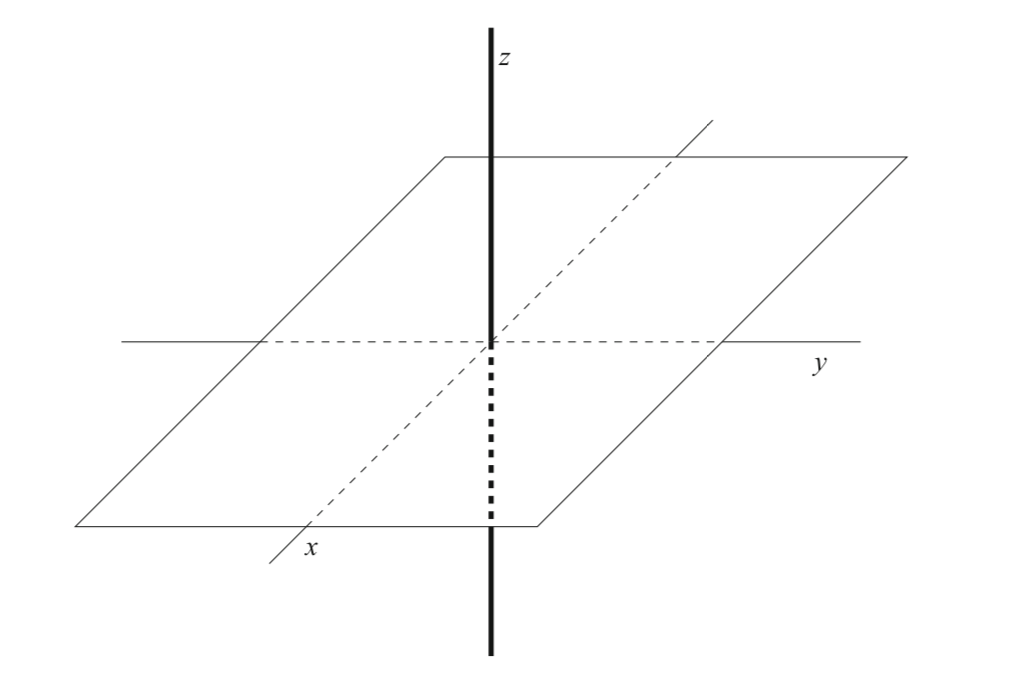
\includegraphics[width=1.0\textwidth]{affineVariety.png}
 	\caption[Example of an affine variety]{Affine variety defined by $(xz,yz)$. Image source: (\cite{algGeom}, page $9$).}
 	\label{fig1}
 \end{figure}

 \begin{DF}
Let $R$ be a commutative ring, then any non-empty subset $I \subseteq R$ is called a (two-sided) \textbf{ideal} of $R$ if it satisfies following requirements:
\begin{itemize}
\item $I \neq \emptyset,$\hfill ($I$ is a non-empty set)
\item $\forall f,g \in I: (f + g) \in I,$ \hfill ($I$ is closed under addition)
\item $\forall f \in I,\ \forall h \in R: hf \in I.$ \hfill ($I$ is closed under multiplication by $R$)
\end{itemize}
\end{DF}
\noindent This thesis is predominantly concerned with the ideals generated by a finite number of polynomials over a finite field.
\begin{DF}
Let $X = (x_1, \ldots ,x_n)$ be an ordered $n$-tuple of formal variables and let $f_1,\ldots,f_s \in \mathbb{F}[X] $ be an $s$-tuple of polynomials. Then the set
$$
\langle f_1, \ldots, f_x \rangle := \bigg\{ \sum_{i=1}^n h_if_i\ |\ h_1,\ldots,h_s \in \mathbb{F}[X]\bigg\}
$$
\end{DF}
\noindent is called the \textbf{ideal generated by} polynomials $f_1,\ldots,f_s$.
\begin{RM}
Every ideal $I$ of $\mathbb{F}[X]$ is finitely generated, which means:
$$
\exists s \in \mathbb{N},\ \exists f_1,\ldots,f_s \in \mathbb{F}[X]: I = \langle f_1, \ldots, f_s \rangle,
$$
\noindent and we say that the polynomials $f_1,\ldots,f_s$ form a \textbf{basis} of $I$. Note that a given ideal $I$ may have many different bases. If we have two different bases $B_1 = (f_1,\ldots,f_s),\ s \in \mathbb{N},$ and $B_2 = (g_1, \ldots, g_t),\ t \in \mathbb{N},$ of the same ideal $I$ in $\mathbb{F}[X]$, such that $I = \langle B_1\rangle = \langle B_2 \rangle,$ then the affine varieties ${\text{in }\mathbb{F}^n}$, defined by the bases $B_1$ and $B_2$, are the same.
$$
\mathcal{V}(B_1) = \mathcal{V}(B_2).
$$
\end{RM}
\begin{theorem}
Let $\mathcal{V} \subseteq \mathbb{F}^n$ be an affine variety and let $X = (x_1, \ldots ,x_n)$ be an ordered $n$-tuple of formal variables. Then the set 
$$
\mathbf{I}(\mathcal{V}) := \{ f \in \mathbb{F}[X]\ |\ \forall a \in \mathcal{V}: f(a) = 0\}.
$$
is an ideal of $\mathbb{F}[X]$.
\end{theorem}
\begin{DF}
The ideal $\mathbf{I}(\mathcal{V})$ is called the \textbf{ideal of affine variety} $\mathcal{V}$.
\end{DF}
\begin{RM}
The natural question to ask is whether $\mathbf{I}(\mathcal{V}(f_1,\ldots,f_s)) = \langle f_1,\ldots,f_s \rangle.$ The answer, unfortunately, is not always yes, but the following inclusion holds:
$$
\langle f_1,\ldots,f_s \rangle \subseteq \mathbf{I}(\mathcal{V}(f_1,\ldots,f_s)) .
$$
\end{RM} 
\begin{theorem}
Let $f,g \in \mathbb{F}[x]$ be two non-constant polynomials of degrees $l,m \in \mathbb{Z}_{>0}$, deg$(f) = l,\ $deg$(g)=m$. Then $f,g$ have a common factor in $\mathbb{F}[x]$ if and only if there are polynomials $A,B \in \mathbb{F}[x]$, such that:
\begin{enumerate}
\item $A \neq 0,\ B \neq 0,$ 
\item deg$(A) \leq m - 1,$ deg$(B) \leq l - 1,$
\item $Af  + Bg = 0.$
\end{enumerate}
\noindent To decide whether polynomials $f,g$ have a common factor, we can rewrite $Af  + Bg = 0$ as a system of linear equations and find a non-zero solution.
\begin{align*}
A &= u_0x^{m-1} + \cdots + u_{m-1}, \\
B &= v_0x^{l-1} + \cdots + v_{l-1}, \\
f &= c_0x^l + \cdots + c_l, \quad c_0 \neq 0, \\
g &= d_0x^m + \cdots + d_m, \quad d_0 \neq 0. \\
\end{align*}
If we compare the coefficients of powers of $x$, we get a system of linear equations with variables $u_i,\ i \in \{0,1,\ldots	, m - 1\}$ and $v_j,\ j \in \{0,1,\ldots, l - 1\}$ and coefficients $c_i, d_j \in \mathbb{F}.$ The coefficient matrix of this system is called the \textbf{Sylvester matrix} of $f$ and $g$ with respect to $x$, denoted by Syl$_{x}(f,g)$. Syl$_{x}(f,g)$ is the following $(l + m) \times (l + m)$ matrix:
$$
\text{Syl}_{x}(f,g) := \begin{pmatrix}
c_0 &  &  &  &             d_0 &  &  &  \\
c_1 & c_0 &  &  &        d_1 & d_0 &   &  \\
c_2 & c_1 & \ddots &  & d_2 & d_1 & \ddots  &  \\
\vdots & & \ddots & c_0 & \vdots &  & \ddots & d_0 \\
 &  \vdots &  & c_1 &  & \vdots &  & d_1 \\
c_l &  &  &  &  d_m&  &  & \\
 & c_l &  & \vdots &  & d_m &  & \vdots \\
 &  & \ddots &  &  &  & \ddots &  \\
\coolunder{m \text{ columns}}{\hphantom{..} & \hphantom{...} & \hphantom{..}  & c_l & }\coolunder{l \text{ columns}}{\hphantom{...} & \hphantom{...} & \hphantom{......} & d_m \hphantom{..}} \\
\end{pmatrix},
$$ \\  \\
\noindent where the empty spaces are filled by zeros.
\end{theorem}
\begin{DF}
\noindent The determinant of the Sylvester matrix is called the \textbf{resultant} of polynomials $f$ and $g$ with respect to $x$, and is denoted by Res$_{x}(f,g)$.
\end{DF}
\noindent Furthermore, $f,g$ have a common factor in $\mathbb{F}[x]$ if and only if Res$_x(f,g) = 0$, which is equivalent to the above-presented system of linear equations having a non-zero solution. An example of the resultant of two quadratic polynomials is shown on page \pageref{resExample}. 
\\ \\
\noindent If $f,g$ have a common factor $h \in \mathbb{F}[x],\ \text{deg}(h) \geq 1$, then there exist ${f_1, g_1 \in \mathbb{F}[x]}$, such that:
$$
f = hf_1, \quad g = hg_1.
$$
\begin{theorem}
\noindent Let $\mathbb{F}$ be an algebraically closed field, let polynomials $f,g$ have a common factor $h \in \mathbb{F}[X]$, deg$(h) \geq 1$. Since $\mathbb{F}$ is an algebraically closed field, a (non-constant) common factor $h$ has a root ${r \in \mathbb{F}}$: ${h(r) = 0}$. Therefore, $r$ is a common root of polynomials $f,g$:
\begin{align*}
(hf_1)(r) &= h(r)f_1(r) = 0f_1(r) = 0 \implies f(r) = 0 ,\\
(hg_1)(r) &= h(r)g_1(r) = 0g_1(r) = 0 \implies g(r) = 0.\\
\end{align*}
\end{theorem}
\subsection{Monomial Ordering}
\noindent The notion of ordering of terms in a polynomial is a key ingredient in many algorithms, e.g. the long division of polynomials. When dealing with polynomials in only one variable, we usually write the terms of the polynomial in the decreasing order by their monomial degree. \\ \\

\noindent We would like to establish an ordering on the terms in polynomials in $\mathbb{F}[X],$ where $X = (x_1, \ldots, x_n)$. First, we note that we can reconstruct the monomial $X^{\alpha} = x_1^{\alpha_1}\cdots x_n^{\alpha_n}$ from the $n$-tuple of exponents $\alpha = (\alpha_1,\ldots, \alpha_n) \in \mathbb{Z}_{\geq 0}^n.$ Based on this observation, we define an ordering $>$ on the space $\mathbb{Z}_{\geq 0}^n$ which also gives us an ordering on the monomials $\in \mathbb{F}[X].$ If for some $\alpha, \beta \in  \mathbb{Z}_{\geq 0}^n$ and some ordering $>$ holds: $\alpha > \beta$ we also say that $X^\alpha > X^\beta.$ In this thesis, we only consider \textbf{total orderings}, which means that for every pair of monomials $X^\alpha$ and $X^\beta$ exactly one of the three statements holds:
\begin{itemize}
\item $X^\alpha > X^\beta,$\hfill (when $\alpha > \beta$)
\item $X^\alpha = X^\beta,$\hfill (when $\alpha = \beta$)
\item $X^\alpha < X^\beta,$\hfill (when $\alpha < \beta$)
\end{itemize}
\noindent and $>$ is transitive:
$$
\forall \alpha, \beta, \gamma \in \mathbb{Z}_{\geq 0}^n: (X^\alpha > X^\beta \land X^\beta > X^\gamma) \implies X^\alpha > X^\gamma.
$$
\noindent We also require that multiplication of two polynomials does not change the relative ordering of terms. Therefore, the following property for $>$ must hold:
$$
\forall \alpha, \beta, \gamma \in \mathbb{Z}_{\geq 0}^n: X^\alpha > X^\beta \implies X^\alpha X^\gamma > X^\beta X^\gamma.
$$
\noindent Which in terms of the exponent vectors means: 
$$
\forall \alpha, \beta, \gamma \in \mathbb{Z}_{\geq 0}^n: \alpha > \beta \implies \alpha + \gamma > \beta + \gamma.
$$
\noindent To summarize all the requirements, we make the following definition.
\begin{DF}
A \textbf{monomial ordering} $>$ on $\mathbb{F}[X]$, where $X = (x_1, \ldots, x_n)$, is a relation $>$ on $\mathbb{Z}_{\geq 0}^n$ satisfying:
\begin{itemize}
\item $>$ is a total ordering on $\mathbb{Z}_{\geq 0}^n$,
\item $\forall \alpha, \beta, \gamma \in \mathbb{Z}_{\geq 0}^n: \alpha > \beta \implies \alpha + \gamma > \beta + \gamma,$
\item $\forall A \subseteq \mathbb{Z}_{\geq 0}^n,\ A \neq \emptyset: \exists \alpha \in A,\ \forall \beta \in A \setminus \{\alpha \}: \beta > \alpha.$ 
\end{itemize}
\noindent The last requirement demonstrates, that in every non-empty subset of $\mathbb{Z}_{\geq 0}^n$ there exists a minimum element under the relation $>$.
\end{DF}
\begin{DF}
Let $\alpha = (\alpha_1, \ldots, \alpha_n),\ \beta = (\beta_1, \ldots, \beta_n)\in \mathbb{Z}_{\geq 0}^n.$ \textbf{Lexicographic Order} (\textbf{lex}), denoted by $>_{lex}$, is a generalisation of the way words are ordered in a dictionary. We say $\alpha >_{lex} \beta$ if the leftmost non-zero entry of the vector difference $\alpha - \beta \in \mathbb{Z}^n$ is positive. We write: $X^\alpha >_{lex} X^\beta$ if $\alpha >_{lex} \beta$.
\end{DF}
For example:
\begin{itemize}
\item $(10,4,3) >_{lex} (10, 3, 4),$ since $\alpha - \beta = (0,1,-1)$.
\item $(7,5,3,1) >_{lex} (7, 5, 2, 4),$ since $\alpha - \beta = (0,0,1,-3)$.
\item The variables $x_1,\ldots,x_n$ are ordered in the usual way by the lexicographic order:
$$
(1,0,\ldots,0) >_{lex} (0,1,0,\ldots, 0) >_{lex} \cdots >_{lex} (0, \ldots, 0, 1),
$$
so $x_1 >_{lex} x_2 >_{lex} \cdots >_{lex} x_n.$ \\ \\
In the rest of this thesis, we assume $x >_{lex} y >_{lex} z,$ unless stated otherwise.
\end{itemize} 
\begin{DF}
Let $\alpha = (\alpha_1, \ldots, \alpha_n),\ \beta = (\beta_1, \ldots, \beta_n)\in \mathbb{Z}_{\geq 0}^n.$ \textbf{Graded Lexicographic Order} (\textbf{grlex}), denoted by $>_{grlex}$, at first orders the terms by the total degree, then it breaks ties using the standard lexicographic order defined above. 
$$
\alpha >_{grlex} \beta: (|\alpha| > |\beta|) \lor (|\alpha| = |\beta| \land \alpha >_{lex} \beta),
$$
where $|\alpha| = \sum_{i=1}^n \alpha_i$ and $|\beta| = \sum_{i=1}^n \beta_i$.
\end{DF}
\begin{itemize}
\item $(10,2,6) >_{grlex} (10, 3,4),$ since $|\alpha| = 18 > |\beta| = 17$.
\item $(7,5,3,1) >_{grlex} (7, 5, 2, 4),$ since $|\alpha| = 16 = |\beta|$ and $\alpha >_{lex} \beta$.
\item The variables $x_1,\ldots,x_n$ are ordered in the same way as by $>_{lex}$ order:
$$
(1,0,\ldots,0) >_{grlex} (0,1,0,\ldots, 0) >_{grlex} \cdots >_{grlex} (0, \ldots, 0, 1),
$$
\end{itemize} 
\begin{DF}
Let $\alpha = (\alpha_1, \ldots, \alpha_n),\ \beta = (\beta_1, \ldots, \beta_n)\in \mathbb{Z}_{\geq 0}^n.$ \textbf{Graded Reverse Lexicographic Order} (\textbf{grevlex}), denoted by $>_{grevlex}$. We say $\alpha >_{grevlex} \beta$ if $|\alpha| > |\beta|$ or if $|\alpha| = |\beta|$ and the rightmost non-zero entry of vector difference $\alpha - \beta \in \mathbb{Z}^n$ is negative.
\end{DF}
\begin{RM}
Grevlex is somehow a less intuitive order, however, it is usually the most efficient for computations.
\end{RM}
\begin{itemize}
\item $(4,7,1) >_{grevlex} (4, 2,5),$ since $|\alpha| = 12 > |\beta| = 11$.
\item $  (7, 5, 1, 3) >_{grevlex} (1,5,3,7),$ since $|\alpha| = 16 = |\beta|$, \\
and $\alpha - \beta = (6,0,-2, -4),\ -4 < 0$.
\item The variables $x_1,\ldots,x_n$ are ordered in the same way as by $>_{lex}$ order:
$$
(1,0,\ldots,0) >_{grevlex} (0,1,0,\ldots, 0) >_{grevlex} \cdots >_{grevlex} (0, \ldots, 0, 1),
$$
\end{itemize}
Here we illustrate how the polynomial $f(x,y,z) = 4xy^2z + 4z^2 - 5x^3 + 7x^2z^2 \in \mathbb{Z}[x,y,z]$ would be written, if we reorder its terms by a monomial ordering in decreasing order:
\begin{itemize}
\item With respect to the lex order:
$$
f(x,y,z) = -5x^3 + 7x^2z^2 + 4xy^2z + 4z^2.
$$
\item With respect to the grlex order:
$$
f(x,y,z) = 7x^2z^2  + 4xy^2z -5x^3 + 4z^2.
$$
\item With respect to the grevlex order:
$$
f(x,y,z) = 4xy^2z + 7x^2z^2  -5x^3 + 4z^2.
$$
The first two terms have the same total degree of $4$ and $xy^2z >_{grevlex} x^2z^2$ because $(1,2,1) - (2,0,2) = (-1,2,-1)$ and $-1 < 0$.
\end{itemize} 
\begin{DF}
Let $f = \sum_\alpha a_\alpha X^\alpha$ be a non-zero polynomial in $\mathbb{F}[X]$, and let $>$ be a monomial order.
\begin{itemize}
\item The \textbf{multidegree} of $f$ is:
$$
\text{multideg}(f) := \text{max}(\alpha \in \mathbb{Z}_{\geq 0}^n\ |\ a_\alpha \neq 0),
$$
the maximum is taken with respect to $>$.\\ \\
\item The \textbf{leading coefficient} of $f$ is:
$$
\text{LC}(f) := a_{\text{multideg}(f)} \in \mathbb{F}.
$$
\item The \textbf{leading monomial} of $f$ is:
$$
\text{LM}(f) := X^{\text{multideg}(f)} \in \mathbb{F}[X],
$$
with coefficient $1$.
\item The \textbf{leading term} of $f$ is:
$$
\text{LT}(f) := (\text{LC}(f)\cdot \text{LM}(f)) \in \mathbb{F}[X].
$$
\end{itemize}
\end{DF}
\noindent To illustrate these notions, let $f(x,y,z) = 4xy^2z + 4z^2 - 5x^3 + 7x^2z^2 \in \mathbb{Z}[x,y,z]$ as before and let us use $>_{grevlex}$ order.
\begin{align*}
f(x,y,z) &= 4xy^2z + 7x^2z^2  -5x^3 + 4z^2, \text{ (in  grevlex order)}\\
\text{multideg}(f)&=(1,2,1), \\
\text{LC}(f)&=4, \\
\text{LM}(f)&=xy^2z, \\
\text{LT}(f)&=4xy^2z. \\
\end{align*}
Now we can formulate the idea of a general division algorithm in $\mathbb{F}[X]$.
\begin{DF}
Let $p, q \in \mathbb{F}[X]$ be two monomials, we say the monomial $p$ is \textbf{divisible} by the monomial $q$ if and only if there exists a monomial $h \in \mathbb{F}[X]$, such that: $p = qh$. We denote it by $q\ |\ p$ and read it as \textbf{$\mathbf{q}$ divides $\mathbf{p}$}.
\end{DF}
\begin{theorem}
Let $>$ be a monomial order on $\mathbb{Z}_{\geq 0}^n$, let $F = (f_1, \ldots, f_s)$ be an ordered $s$-tuple of polynomials in $\mathbb{F}[X],$ where $X = (x_1, \ldots, x_n)$. Then every $f \in \mathbb{F}[X]$ can be written as:
$$
f = q_1f_1 + \cdots + q_sf_s + r,
$$
where $q_i, r \in \mathbb{F}[X]$, and either $r = 0$ (is a zero polynomial) or $r$ is a linear combination, with coefficients in $\mathbb{F}$, of monomials $\in \mathbb{F}[X]$ such that none of those monomials is divisible by any of LT$(f_1), \ldots,$LT($f_s$).
\end{theorem}
\begin{DF}
We call the polynomial $r$ from the previous theorem a \textbf{remainder} of $f$ on division by $F$. Furthermore, if $q_if_i \neq 0$, then
$$
\text{multideg}(f) \geq \text{multideg}(q_if_i).
$$
\end{DF}
\noindent We do not describe the division algorithm itself in the thesis, please refer to~\cite{algGeom} on pages 61--68 where the algorithm is discussed in detail.\\ \\
\noindent Unfortunately, the remainder is not unique and depends on the order of the divisors in the set $F$ and also on the monomial order itself. \\ \\
\noindent Moreover, we would like to use this idea to answer the ideal membership problem. Let $f, f_1, \ldots, f_s \in \mathbb{F}[X]$ and let $I = \langle f_1, \ldots, f_s \rangle$ be an ideal. We would like to determine whether $f \in I$. We can clearly state that if the remainder $r$ obtained after division of $f$ by $F = (f_1, \ldots, f_s)$ is $0$, then $f$ has to be an element of the ideal $I$. So $r=0$ is a sufficient condition for the ideal membership. However, it is not a necessary condition for $f$ being in the ideal. To remedy this situation, we try to describe a \textquote{good} basis of the ideal $I$, such that the remainder $r$ on division by the polynomials of this basis is uniquely determined and that the condition $r=0$ is also a necessary condition for $f \in I$. Exactly those are the properties of Gröbner bases, which we describe in the following section.
\section{Gröbner Bases}
Gröbner bases may be used to solve a number of problems concerning polynomial ideals in an algorithmic or computational fashion. It is one of the most commonly used methods for solving systems of multivariate polynomial equations, i.e. calculating the affine variety defined by those polynomial equations. This section is based on~\cite{algGeom}.
\begin{DF}
An ideal $I \subseteq \mathbb{F}[X]$ is called a \textbf{monomial ideal} if there exists a (possibly infinite) subset $A \subseteq \mathbb{Z}_{\geq 0}^n$, such that $I$ consists of all polynomials which are finite sums: $\sum_{\alpha \in A} h_\alpha X^\alpha$, where $h_\alpha \in \mathbb{F}[X].$ We can then write $I$ in the form: $I = \langle X^\alpha \ |\ \alpha \in A\rangle.$ Monomial $X^\beta, \beta \in \mathbb{Z}_{\geq 0}^n,$ lies in the ideal $I$ if and only if there exist $\alpha \in A$, such that $X^\alpha \ |\ X^\beta$ ($X^\beta$ is divisible by some $X^\alpha$). 
\end{DF}
\noindent \textbf{(Dickson's Lemma).} Any monomial ideal ${I = \langle X^\alpha \ |\ \alpha \in A\rangle \subseteq \mathbb{F}[X]}$ can be written in the form $I = \langle X^{\alpha(1)}, \ldots, X^{\alpha(s)}\rangle,\ s \in \mathbb{N},$ where $\alpha(1), \ldots, \alpha(s) \in A$. In particular, $I$ has a finite basis $(X^{\alpha(1)}, \ldots, X^{\alpha(s)})$.
\begin{theorem}
A monomial ideal $I \subseteq \mathbb{F}[X]$ has a finite basis $(X^{\alpha(1)}, \ldots, $\\$X^{\alpha(s)})$ with the property that $X^{\alpha(i)}$ does not divide $X^{\alpha(j)}$ for any $i \neq j$. Moreover, this basis is unique.
\end{theorem}
\begin{DF}
The unique basis of $I$ from the previous theorem is called the \textbf{minimal basis} of $I$.
\end{DF}
\begin{DF}
Let $I \subseteq \mathbb{F}[X],\ I \neq {0},$ be an ideal and fix a monomial order on $\mathbb{F}[X]$.  Then:
\begin{itemize}
\item We denote by LT$(I)$ the \textbf{set of leading terms} of non-zero elements of~$I$.
$$
\text{LT}(I) = \{ cX^\alpha \ |\ \exists f \in I \setminus \{0\}: \text{LT}(f)= cX^\alpha \}.
$$
\item We denote by $\langle \text{LT}(I) \rangle$ the \textbf{ideal of leading terms} of $I$. $\langle \text{LT}(I) \rangle$ is a monomial ideal, therefore, there exists a finite set $g_1,\ldots, g_t \in I,\ t \in \mathbb{N},$ such that:
$$
\langle \text{LT}(I) \rangle = \langle \text{LT}(g_1), \ldots, \text{LT}(g_t) \rangle.
$$
\end{itemize}
\end{DF}
\noindent Fix a monomial order on $\mathbb{F}[X]$. Then every polynomial $f \in \mathbb{F}[X]$ has a unique leading term.
\begin{DF} A finite subset $G = \{g_1, \ldots, g_t \}$ of an ideal $I \subseteq \mathbb{F}[X],\ I \neq \{ 0 \}$ is said to be a \textbf{Gröbner basis} (or \textbf{standard basis}) if:
$$
\langle \text{LT}(g_1), \ldots, \text{LT}(g_t) \rangle = \langle \text{LT}(I) \rangle.
$$
Additionally, we define the Gröbner basis of the zero ideal $\{0\}$ to be the empty set $\emptyset$ using the convention that $\langle \emptyset \rangle = \{0\}.$
\end{DF}
\begin{RM}
Every ideal $I \subseteq \mathbb{F}[X]$ has a Gröbner basis. Furthermore, any Gröbner basis for an ideal $I$ is a basis of $I$. Gröbner bases for ideals in polynomial rings were introduced by B. Buchberger in his PhD thesis~\cite{bruno}, published in 1965, and named by him in honour of his thesis's advisor W. Gröbner. Buchberger also developed fundamental algorithms to find and work with Gröbner bases. In many computer algebra systems, there is usually used an alternative spelling \textquote{Groebner bases}.
\end{RM}
\phantom{.}
\phantom{.}
\noindent Now we will mention few important properties of Gröbner bases.
\begin{RM}
Let $I \subseteq \mathbb{F}[X]$ be an ideal and let $G = \{g_1, \ldots, g_t\}$ be a Gröbner basis of $I$. Then for any $f \in \mathbb{F}[X],$ there is a unique polynomial $r$ with those two properties:
\begin{itemize}
\item No term of $r$ is divisible by any of LT$(g_1),\ldots,$LT$(g_t)$.
\item $\exists g \in I:\ f = g + r.$
In particular, when using the division algorithm, $r$ is the remainder on division of $f$ by set $G$ no matter how are the elements of $G$ listed.
\end{itemize}
Polynomial $r$ is called the \textbf{normal form} of f. \\ \\ 
\noindent Polynomial $f \in I$ if and only if the remainder $r$ on division $f$ by $G$ is zero, $r = 0.$
\end{RM}
\begin{NRM}
Let $f \in \mathbb{F}[X]$ be a polynomial and let $F = (f_1, \ldots, f_s) \subseteq \mathbb{F}[X]$ be an ordered $s$-tuple of polynomials. We denote the remainder on the division of $f$ by $F$ by $\overline{f}^F$. If $F$ is a Gröbner basis of $\langle f_1, \ldots, f_s \rangle$, then we can regard $F$ as a set without any particular order because the remainder on the division by a Gröbner basis is unique.
\end{NRM}
\begin{DF}
Let $f,g \in \mathbb{F}[x_1,\ldots,x_n]$ be non-zero polynomials. Let $\alpha = \text{multideg}(f)$, $\beta = \text{multideg}(g)$ and ${\gamma = (\gamma_1,\ldots,\gamma_n)},$ where ${\gamma_i = \text{max}(\alpha_i,\beta_i)}$ for each $i \in \{1,\ldots,n\}.$ We call $X^\gamma$ the \textbf{least common multiple} of LM$(f)$ and LM$(g)$ and denote it by $X^\gamma = \text{lcm(LM}(f),(\text{LM}(g)).$ \\ \\
\noindent The \textbf{S-polynomial} of $f$ and $g$ is the combination:
$$
\text{S}(f,g) := \frac{X^\gamma}{\text{LT}(f)}\cdot f - \frac{X^\gamma}{\text{LT}(g)}\cdot g.
$$
\end{DF}
\noindent For example, let $f=x^3y^2 - x^2y^3 + x$ and $g = 3x^4y + y^2$ in $\mathbb{R}[x,y]$ with grlex order. Then $\gamma = (4,2)$ and
\begin{align*}
\text{S}(f,g) &= \frac{x^4y^2}{x^3y^2}\cdot f - \frac{x^4y^2}{3x^4y}\cdot g \\
&= x\cdot f - \frac{1}{3}y^3\cdot g \\
&= -x^3y^3 + x^2 - \frac{1}{3}y^3.
\end{align*}
An S-polynomial is \textquote{designed} to produce cancellation of the leading terms.
\begin{DF}
\textbf{(Buchberger's Criterion)}: Let $I$ be a polynomial ideal. Then a basis $G = \{g_1,\ldots,g_t\}$ of $I$ is a Gröbner basis of $I$ if and only if for all pairs $i\neq j$, the remainder on division by S$(g_i,g_j)$ by $G$ (listed in some order) is zero.
\end{DF}
\noindent Let $G$ be a set of generators, Buchberger's algorithm transforms this set to a Gröbner basis of the polynomial ideal generated by $G$. In essence, the S-polynomials of pairs of generators are repeatedly computed and then divided by the set of generators. If the remainder of this division is non-zero, then we add this remainder to the set of generators. We repeat this process until no new elements are added to the set of generators, i.e. the Buchberger's Criterion is fulfilled. Detailed description of this algorithm is on page 91 in~\cite{algGeom}.
\begin{DF}
A \textbf{reduced Gröbner basis} for a polynomial ideal $I$ is a Gröbner basis $G$ for $I$ such that:
\begin{itemize}
\item $\forall p \in G: \text{LC}(p) = 1.$
\item $\forall p \in G$: no monomial $p$ lies in $\langle\text{LT}(G \setminus \{p\}) \rangle.$
\end{itemize}
\end{DF}
\noindent Any polynomial ideal $I\neq \{\emptyset\}$ for a given monomial order has a unique reduced Gröbner basis. 
\\
\\
\noindent Now we describe, how to use Gröbner bases for finding all the solutions of a system of multivariate polynomial equations.
\begin{DF}
Given ideal $I = \langle f_1,\ldots,f_s\rangle \subseteq \mathbb{F}[x_1,\ldots,x_n]$, the $l$-th \textbf{elimination ideal} $I_l$ is the ideal of $\mathbb{F}[x_{l+1},\ldots,x_n]$ defined by:
$$
I_l := I \cap \mathbb{F}[x_{l+1},\ldots,x_n].
$$
\end{DF}
\noindent Note that different orderings of the variables lead to different elimination ideals.
\begin{theorem}
\textbf{(The Elimination Theorem).} Let $I \subseteq \mathbb{F}[x_1,\ldots,x_n]$ be an ideal and let $G$ be a Gröbner basis of $I$ with respect to lex order where $x_1 > x_2 > \cdots > x_n$. Then, for every $0\leq l \leq n$, the set:
$$
G_l := G \cap \mathbb{F}[x_{l+1},\ldots,x_n]
$$
is a Gröbner basis of the $l$-th elimination ideal $I_l$.
\end{theorem}
\vphantom{.}
\noindent Given an ideal $I = \langle f_1,\ldots,f_s \rangle$, we wish to find all the points that lie in the affine variety $\mathcal{V}(I)$. We build up the solutions one coordinate at a time. At first, we find the affine variety $\mathcal{V}(I_{n-1})$, which is equivalent to finding the roots of a univariate polynomial in $\mathbb{F}[x_n]$. We call any solution $(a_n) \in \mathcal{V}(I_{n-1})$ a \textbf{partial solution} of the original system of equations. The next step is to extend a partial solution $(a_n)$ to a partial solution $(a_{n-1},a_n) \in \mathcal{V}(I_{n-2})$. To do that, we substitute $(a_n)$ into all the polynomial equations in $I_{n-2}$. Thereafter, we obtain a univariate polynomial equation in $\mathbb{F}[x_{n-1}]$, which we can conveniently solve. Note that not every partial solution in $\mathcal{V}(I_{n-1})$ extends to a partial solution in $\mathcal{V}(I_{n-2})$. We repeat this process until we find $\mathcal{V}(I_0) = \mathcal{V}(I)$, a set of all \textbf{complete solutions} of the original system of equations.
\begin{DF}
Let $I \subset \mathbb{F}[X]$ be a polynomial ideal over a finite field $\mathbb{F}$. We say $I$ is a zero-dimensional ideal if and only if the affine variety $\mathcal{V}(I)$ is a finite set over every field $\mathbb{T}$ such that $\mathbb{F} \subseteq\mathbb{T}$.
\end{DF}
\begin{DF}
\label{triagForm}
Let $G = \{g_1,\ldots,g_s\}$ be the reduced Gröbner basis for a zero-dimensional ideal $I \subset \mathbb{F}[x_1,\ldots,x_n]$ with respect to the lexicographic order of monomials with $X_1 >_{\text{lex}} \cdots >_{\text{lex}} X_n$. Additionaly, let $G$ be ordered so that every LT$(g_j) >_{\text{lex}} $LT($g_{j+1}$). Then for each $i \in \{1,\ldots,n\}$ there exists $j=j(i)$ for which LT$(g_j)=x_i^{d_i}$ for some $d_i > 0.$ This is called the \textbf{triangular form} and is especially convenient for finding all the points that lie in the affine variety defined by the polynomials $g_1,\ldots,g_n$. The last polynomial in $G$ is univariate: $g_s = g_s(X_n)$. We can find its roots (a partial solution) and substitute them into all the other polynomials in $G$. After such substitution, at least one of the earlier polynomials $g_i,\ i \in \{1,\ldots,s-1\}$ is univariate in $X_{n-1}$. We can repeat this process until we find the affine variety $\mathcal{V}(G)$, the set of all complete solutions. This method is called \textbf{backsolving} or \textbf{back-substitution}, for more information see~\cite{week11}.
\end{DF}

\chapter{Elliptic Curves and the Discrete Logarithm Problem}\label{ch2}
In this chapter, we revise the theory of elliptic curves and state the elliptic curve discrete logarithm problem (ECDLP). In the last section, we also introduce the reader to the concept of summation polynomials, which are the primary building blocks in many specialised algorithms (exploiting the particular group structure) solving the ECDLP. Examples of such algorithms are discussed in detail in chapter~\ref{specAlg}.
\section{Elliptic Curves}
This section focuses on elliptic curves over finite fields and groups of their points. At first, we define what is a general elliptic curve. Afterwards, we show how to define an Abelian group on the set of points of an elliptic curve. This section is based mostly on~\cite{mky}.
\begin{DF}
An \textbf{elliptic curve} over a (prime order) finite field $GF(p),$ \\ $p > 3,\ p$ prime, defined by the short Weierstrass equation, is a set:
$$
E(GF(p)) := \{(x,y)\ |\ x,y \in \mathbb{F},\ y^2 = x^3 + Ax+B\} \cup \{ \mathcal{O} \},
$$
where $A, B \in GF(p)$ are \textbf{coefficients of the elliptic curve}. Coefficients $A,B$ have to satisfy the following condition: $4A^3 + 27B^2 \neq 0$, which guarantees the right-hand side polynomial $f(x)=x^3 + Ax+B$ has 3 distinct roots. Elliptic curves are \textbf{non-singular} curves, i.e. they do not have any cusps nor self-intersections. Point $\mathcal{O}$ is called the \textbf{point at infinity} (in the projective plane).
\end{DF}
\begin{DF}
Let $E(GF(p))$ be an elliptic curve, and let $P,Q \in E(GF(p)),$\\${P=(x_1,y_1),\ Q=(x_2,y_2)}$ be two points on the elliptic curve $E$. We define the binary operation $\oplus: E(GF(p)) \times E(GF(p)) \to E(GF(p))$, called \textbf{addition on the elliptic curve} $E(GF(p))$, as follows:
\begin{itemize}
\item If $P = \mathcal{O},\ P \oplus Q = Q,$ or if $Q = \mathcal{O},\ P \oplus Q = P.$ Therefore, the point at infinity $\mathcal{O}$ is an identity element of the operation $\oplus$.
\item Else if $x_1 = x_2$ and $P\neq Q$, $P\oplus Q = \mathcal{O}.$ Point at infinity $\mathcal{O}$ is the identity element of operation $\oplus$. Therefore, point $Q$ is the \textbf{additive inverse} of point $P$, denoted by $\ominus P$. We now state the explicit formula for point $\ominus P$, we know its $x$-coordinate is $x_1$. We use the elliptic curve equation and substitute $X$ with $x_1$:
$$
Y^2  = (x_1^3 + Ax_1 + B),
$$
which is a quadratic equation in the variable $Y$. Since we already know one of its roots $y_1$, the other root has to be $-y_1$. Hence
$$\ominus P = (x_1, -y_1).$$
\item a) Else if $x_1 \neq x_2$, let $\lambda$ be the slope of the line defined by the points $P,Q.$
$$
\lambda = \frac{y_2 - y_1}{x_2 - x_1},
$$
b) Else if $P = Q$ (\textbf{point doubling}), let $\lambda$ be the slope of the tangent line to the elliptic curve equation at the point $P.$
$$
\lambda = \mathlarger{\mathlarger{\frac{\frac{\partial E}{\partial X}}{\frac{\partial E}{\partial Y}}}}(x_1, y_1) = \frac{3x_1^2+ A}{2y_1}, 
$$
where $\partial E/\partial X$ and  $\partial E/\partial Y$ are the partial derivatives of the elliptic curve equation with respect to $X,Y$ in particular. \\ \\
\noindent The result of the operation $\oplus$ is:
\begin{align*}
x_3 &= \lambda^2 - x_1 - x_2, \\
y_3 &= \lambda(x_1 - x_3) - y_1, \\ 
 P \oplus Q &= (x_3, y_3).
\end{align*}
\end{itemize}
\end{DF}
\begin{theorem}
A set of points on the elliptic curve defined by the short Weierstrass equation and the binary operation $\oplus$ form an Abelian group $(E(GF(p)), \oplus)$. We denote it by $E(p)$. If we want to explicitly mention the coefficients $A,B$, then we use $E_{A,B}(p)$.
\end{theorem}
\begin{NRM}
Let $P \in E(p)$ be a point on an elliptic curve $E$ over $GF(p)$. To shorten the notation of the repeated application of the group law, we use the notation introduced in chapter 1. To remind our readers; \textbf{multiplication} of a point on the elliptic curve $E$ by an integer $t$ has the following meaning:
$$
\forall P \in E(p),\ \forall t \in \mathbb{Z}: tP := \begin{cases} \underbrace{P \oplus P \oplus \cdots \oplus P}_{\text{$t$-times}} &\quad t > 0, \\
\mathcal{O} \text{ (identity element) } &\quad t = 0, \\
\underbrace{(\ominus P) \oplus (\ominus P) \oplus \cdots \oplus (\ominus P)}_{\text{$t$-times}} &\quad t < 0.
\end{cases}
$$
\end{NRM}
\begin{theorem}\textbf{(Hasse's Theorem.)} \label{hase}Let $E$ be an elliptic curve over a finite field $GF(p),\ p$ prime. Then the following inequalities hold:
$$
p + 1 -2\sqrt{p} \leq \#E(p) \leq p + 1 + 2\sqrt{p}.
$$
In other words, the number of points of the elliptic curve group $E(p)$ is close to the prime $p$. To calculate the exact number of points in $E(p)$, the Schoof-Elkies-Atkin's (SEA) algorithm is commonly used. The time complexity of the SEA algorithm amounts to $O(\log^{2\mu + 2}(p))$ bit operations, where $\mu$ is a constant such that two $T$-bit integers can be multiplied in time $T^\mu$, and the space complexity is $O(\log^2(p)).$ The detailed description of the SEA algorithm can be found in chapter 17 of~\cite{handbook}. 
\end{theorem}
\subsection{Complexity of Arithmetic Operations on an Elliptic Curve} 
The complexity of arithmetic operations on $E$ is based on the complexity of operations in the underlying finite field $GF(p)$. The exact number of arithmetic operations depends on the used algorithm, its implementation and on the architecture of the CPU where the particular code is executed. Table~\ref{tblComp} provides a brief summary of the relationship between the operations on elliptic curve $E$ and the number of arithmetic operations in the underlying finite field $GF(p)$. Addition in $GF(p)$ is denoted by $+_p$, multiplication in $GF(p)$ is denoted by $\cdot_p$, and the last column of table~\ref{tblComp} is the number of multiplicative inverses in $GF(p)^{\times}$.
\begin{table}[H]
\centering
\begin{tabular}{ |c||c|c|c| } 
 \hline
 & \# $+_p$ & \# $\cdot_p$ & \# mult. inverses \\ 
 \hline
 \hline
$\ominus P$ & 1 & 0 & 0  \\  \hline
$P \oplus Q, P \neq Q$ & 6 & 3 & 1 \\  \hline
$P \oplus Q, P = Q$ & 5 & 5 & 1 \\  \hline
$tP,\ t \in \mathbb{Z}_{\geq 0},\ k = \mathlarger{\lceil} \log_2(t) \mathlarger{\rceil}$\footnotemark & $ (5k + 3k)$ & $(5k + 1.5k)$ & $(k + 0.5k)$ \\ \hline
\end{tabular}
\caption[Complexity of arithmetic operations on $E$]{Complexity of arithmetic operations on the elliptic curve $E$ over a finite field $GF(p)$.}
\label{tblComp}
\end{table}
\footnotetext{Using signed binary expansion of $t$ for the double-and-add algorithm, see~\cite{mky} page 105.}
\noindent We denote the number of bits of $p$ by $n = \mathlarger{\lceil} \log_2(p) \mathlarger{\rceil}$. Addition in $GF(p)^{+}$ is asymptotically $O(n)$, multiplication in $GF(p)^{\times}$, using Montgomery method~\cite{handbook}, is $O(n^2)$ and the calculation of a multiplicative inverse in $GF(p)^{\times}$, using a careful implementation of the extended Euclidean algorithm (EEA)~\cite{handbook}, is $O(n^2)$. An alternative to the EEA for calculating a multiplicative inverse in $GF(p)^{\times}$ is based on Lagrange's theorem (\ref{lagrange}). 
\begin{align*}
\forall a \in GF(p)^{\times},\ \exists n \in \mathbb{N}: \#a \cdot n = \#GF(p)^{\times} &= p - 1, \\ 
\forall a \in GF(p)^{\times},\ \forall n \in \mathbb{N}: a^{\#a \cdot n} = 1 \implies a^{\#a \cdot n - 1} &= a^{-1}, \\
\forall a \in GF(p)^{\times}: a^{-1} &= a^{p-2}.
\end{align*}
To calculate $a^{p-2}$, we can use the standard algorithm called square-and-multiply which has the same complexity $O(n^2)$ as the EEA, for more details see~\cite{mky}.
\section{The Discrete Logarithm Problem}
Suppose that $y = b^x$, given $y,b \in \mathbb{R}_{> 0}$, we are asked to find the exponent $x \in \mathbb{R}$. We can express this problem in the logarithmic form, i.e. $x = \log_b(y)$. $b$ is called the \textbf{base of the logarithm}. To find the unknown $x$, we can use numerical methods that are based on the fact that exponential function is strictly increasing. Therefore, we can guess a random initial solution $x_0$, evaluate $b^{x_0}$ and compare it with $y$. Based on the result of this comparison, we immediately know whether the true solution $x$ is greater, equal, or less than $x_0$. Thus, we can solve this problem over the real numbers efficiently.
\\
\\
\noindent If we were asked to solve the same problem in a finite group instead, the situation would be significantly more complicated.
\begin{DF}
Let $G = (M, \cdot)$ be an Abelian group and let $h = g^x$, given $h \in \langle g \rangle$ and the base $g \in M$, we are asked to find the exponent $x$~$\in$~$\{0,1, \ldots, \#g - 1\}.$ We call $x$ the \textbf{discrete logarithm} of $h$ with respect to the base $g$, and denote it by $x= \log_g(h)$. The problem of finding the solution $x$ is called the \textbf{discrete logarithm problem} (DLP). We require $h$ to lie in a subgroup generated by $g$ in order to guarantee the existence of the solution to the DLP. 
\end{DF}
\noindent To illustrate the difficulty of solving the DLP, let us consider the multiplicative group $G$ of the finite field $GF(19).$ $G = (\{1,2,\ldots,18\}, \cdot_{19})$ and let us use one of its generators $g=3$ as a base. Group structure is shown in figure~\ref{fig2}. We might be asked to find such $k$ that $3^k \equiv 4 \text{ (mod 19)}$. 
 \begin{figure}[h]
\hspace*{-2cm}
 	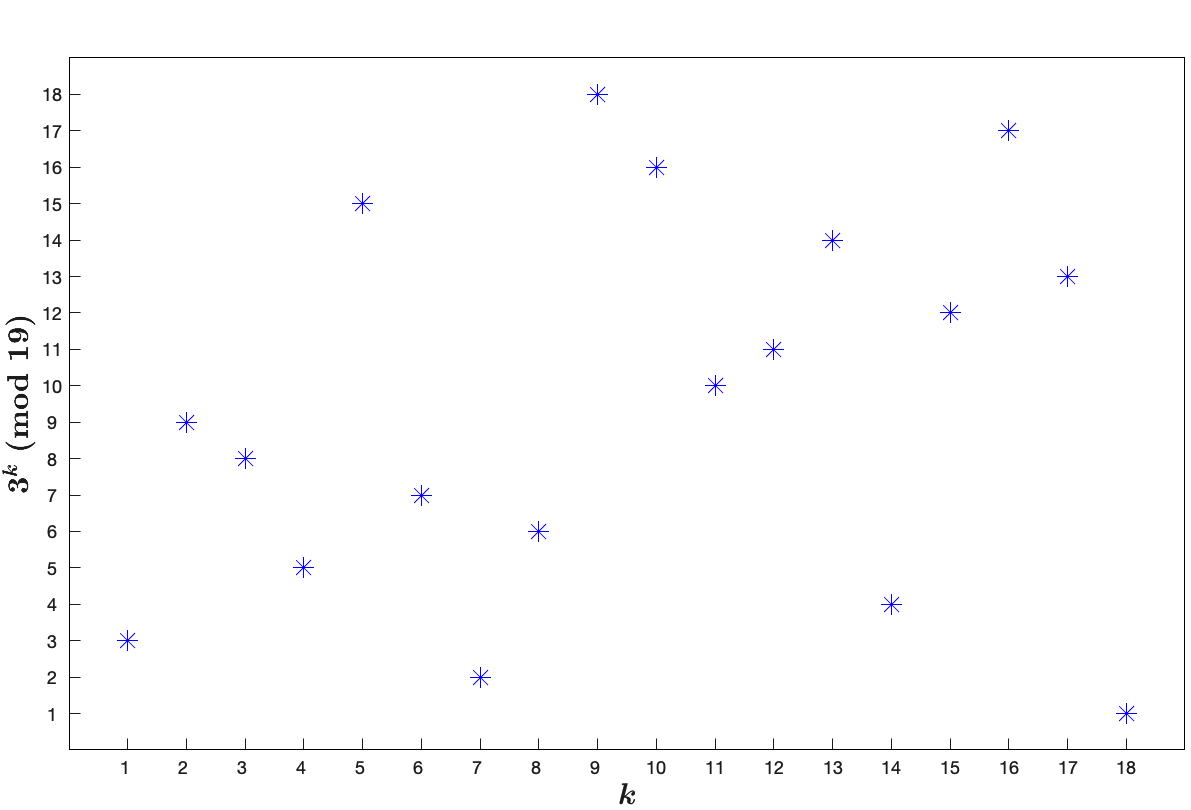
\includegraphics[width=1.25\textwidth]{graph3in19.png}
 	\caption[Example of the group structure of $GF(19)^\times$]{Powers of the generator $g = 3$ in $GF(19)^\times$.}
 	\label{fig2}
 \end{figure}
\noindent Unfortunately, the function $g^k \text{ (mod 19)},\ k \in \mathbb{N},$ is not monotonic. Therefore, we can not use the idea of trying a randomly selected $k_0$ and comparing $3^{k_0} \text{ (mod 19)}$ with $4$, but we can use the fact the group $G$ is finite and its order is $\#G = 18$. We can try all possible values of $k \in \{0, 1, \ldots, 17\}$ and find the solution. This method is called the \textbf{brute-force attack}. 
\begin{align*}
3^0 \equiv 1 \text{ (mod 19)} &\not\equiv 4 \text{ (mod 19)}, \\
3^1 \equiv 3 \text{ (mod 19)} &\not\equiv 4 \text{ (mod 19)}, \\
3^2 \equiv 9 \text{ (mod 19)} &\not\equiv 4 \text{ (mod 19)}, \\
3^3 \equiv 8 \text{ (mod 19)} &\not\equiv 4 \text{ (mod 19)}, \\
&\vdots \quad \vdots \\
3^{13} \equiv 14 \text{ (mod 19)} &\not\equiv 4 \text{ (mod 19)}, \\
3^{14} &\equiv 4 \text{ (mod 19)}.
\end{align*}
Therefore, the solution to this DLP is $k = 14$. We can observe that the brute-force approach is quite lengthy even for a DLP in a group of small order. The complexity of the brute-force attack in a group $G$ is $O(\#G)$ of group operations.
\begin{RM}
Well-known properties of logarithms (over the real numbers) hold for discrete logarithms as well. Let $G$ be a finite Abelian group and let $g \in G$.
\begin{itemize}
\item $\forall p, q \in \langle g \rangle: \log_g(pq) \equiv log_g(p) + log_g(q) \text{ (mod $\#g$)}$,
\item $\forall p, q \in \langle g \rangle: \log_g(p(q)^{-1}) \equiv log_g(p) - log_g(q) \text{ (mod $\#g$)}$,
\item $\forall k \in \mathbb{Z},\ p \in \langle g \rangle: \log_g(p^k) \equiv k \cdot log_g(p) \text{ (mod $\#g$)}$,
\item $\forall h \in \langle g \rangle,\ \#h  = \#g,\ \forall p \in \langle g \rangle: log_g(p) \equiv log_h(p) \cdot log_g(h)  \text{ (mod $\#g$)}$.
\end{itemize}
The last property is the change-of-base formula. It tells us that if we can effectively solve the DLP with respect to some base. We can also use it to effectively solve the DLP with respect to any other base.
\end{RM}

\noindent The discrete logarithm problem can be stated in any group. The difficulty of solving it greatly depends on the group structure and the group operation. To solve the DLP, we can develop a generic algorithm that works in any group and does not exploit the group structure. Alternatively, we can develop a specialised algorithm to tackle the DLP in a specific type of groups. \\\\
\noindent For example, in an additive group $(\{0,1,\ldots, p-1\}, +_p)$, $p$ prime, we can solve the DLP in $O(\log^2(p))$ group operations using the EEA. In 1997, Victor Shoup proved that a generic algorithm to solve the DLP in a generic group of prime order $p$ has to do $O(\sqrt{p})$ group operations~\cite{shoup}. One of the best generic algorithms to match this lower bound is Pollard's $\rho$ (rho)-algorithm, described in subsection~\ref{rhoText}. 
\\
\\
\noindent The main focus of this thesis is to solve the DLP stated on a prime field elliptic curve using a specialised algorithm. 
\begin{DF}
Let $E(p)$ be an elliptic curve over a prime field $GF(p)$, let $P \in E(p)$ and let $Q \in \langle P \rangle$ be another point on $E$. \textbf{Elliptic curve discrete logarithm problem (ECDLP)} is to find an integer $k \in \{0,1,\ldots, \#P - 1\}$ such that $Q = kP$.
\end{DF}
\section{Generic Algorithms for Solving the ECDLP}
In this section, we present the three best known generic algorithms for solving the ECDLP. We use elliptic curve notation. The first algorithm is based on collision finding. Its time complexity matches the Shoup's lower bound; however, the memory requirements are immense. Description of all three algorithms in this section is based on~\cite{mky}.
\subsection{Baby-step Giant-step Algorithm}
\begin{DF}
\textbf{(Baby-step Giant-step (BSGS))}: Let $E(p)$ be an elliptic curve group over $GF(p)$, equipped with operation $\oplus$, let $P \in E$ and $kP = Q \in E(p),\ k \in \{0, 1, \ldots, \#P - 1\}$. We denote the order of $P$ by $N = \#P$. Following algorithm solves the ECDLP in $O(\sqrt{N})$ of group operations $\oplus$.
\begin{itemize}
\item Let $n = \mathlarger{\mathlarger{\mathlarger{\lceil}}} \sqrt{N} \mathlarger{\mathlarger{\mathlarger{\rceil}}}$, we pre-compute a list of length $n$ of multiples of $P$. \\
$0P = \mathcal{O}, P, 2P, \ldots, (n-1)P.$ \hfill (baby-step phase) \\
\item Afterwards, we generate multiples of $Q$ until the first collision with the list generated in the baby-step phase occurs. Let us denote $(-n P) = P'$. \\
$Q \oplus (0P') = Q,\ Q \oplus (1P'),\ \ldots\ ,\ Q \oplus ((n-1)P').$\\
This stage is called the giant-step phase.
\item When the collision occurs for some $i,j$ it means that $iP$ and $Q \oplus (j\cdot P')$ are equal. We can find the solution $k$ to the ECDLP:
\begin{align*}
iP = Q \oplus (j\cdot P') \implies i &\equiv k + (-jn) \text{ (mod $N$)}, \\
k &\equiv i + jn \text{ (mod $N$)}.
\end{align*}
\end{itemize}
\noindent The algorithm is deterministic and is guaranteed to find the solution as it goes over all the possible values of $k$. Every integer in $\{0, 1, \ldots, N - 1\}$ can be expressed as $i + jn,\ n = \mathlarger{\mathlarger{\mathlarger{\lceil}}} \sqrt{N} \mathlarger{\mathlarger{\mathlarger{\rceil}}},\ i,j \in \{0,1,\ldots, n-1\}.$ 
For the efficient implementation, it is crucial to be able to find collision in the pre-computed list effectively. Therefore, it is advisable to use a hash table to store the elements generated in the baby-step phase to achieve the constant time lookup. If that is satisfied, then the algorithm has a time complexity $O(\sqrt{N})$ of group operations. The space complexity of BSGS algorithm is $O(\sqrt{N})$.
\end{DF}
\noindent For example, let $E = E_{1,1}(29)$ be an elliptic curve group over $GF(29)$ defined by the elliptic curve equation $y^2 = x^3 + x + 1$. Let $P = (24,25) \in E$ and let $Q \in \langle P \rangle$ be another point. We want to find an integer $k$ such that $Q = kP.$ The order of $P$ is 36, so we set $n = 6$. The list of points pre-calculated in the baby-step phase is shown in table~\ref{baby}.
\begin{table}[h]
\centering
\begin{tabular}{ |c||c|c|c|c|c|c| }
\hline
$i$ & 0 & 1 & 2 & 3 & 4 & 5\\ \hline
 $iP$ & $\mathcal{O}$ & $(24,25)$ &  $(6,7)$ & $(0,28)$ & $(10,24)$ & $\textbf{(28,12)}$ \\ \hline
\end{tabular}
\caption[List of points pre-calculated in the baby-step phase]{List of points pre-calculated in the baby-step phase.}
\label{baby}
\end{table}
This step depends only on the elliptic curve group $E$ and point $P$. Therefore, we can pre-calculate it only once and reuse it for the calculation of discrete logarithms of different points with respect to the same base point $P$. Let us solve the ECDLP for $Q = (18,15)$. We iterate over the multiples of $Q$ and look for a collision with the pre-calculated list shown in table~\ref{baby}.
\begin{table}[h]
\centering
\begin{tabular}{ |c||c|c|c|c|c|c| }
\hline
$j$ & 0 & 1 & 2 & 3 & 4 & 5\\ \hline
 $Q\oplus(6j\ominus P)$ & $(18,15)$ & $(11,3)$ &  $(12,1)$ & $(8,17)$ & $\mathbf{(28,12)}$ & $(24,4)$ \\ \hline
\end{tabular}
\caption[List of points tried in the giant-step phase]{List of points tried in the giant-step phase.}
\end{table}
\noindent We have found a collision for $j=4$ and $i=5$, found collision is highlighted in bold in both tables. Thus:
$$
5P = Q\oplus(24\ominus P) \implies 4 \equiv k -24 \text{ (mod 36)} \implies k \equiv 29  \text{ (mod 36)}.
$$
We can easily verify that $29P = (18,15) = Q.$
\subsection{Pollard's $\boldsymbol\rho$-Algorithm} \label{rhoText}
\noindent The main drawback of the BSGS algorithm is its space complexity, it needs to store $\sqrt{\#P}$ elliptic curve points. To remedy this problem, in 1978, John Pollard published a different algorithm, which was named after him the Pollard's~$\rho$-algorithm. It has the same time complexity as BSGS, yet the memory requirements are minimal. We first describe Pollard's idea in general, then show how it can be applied to solve the ECDLP.
\begin{theorem}
\label{pol}
 \textbf{(Pollard's $\boldsymbol\rho$-algorithm)}: Let $S$ be a finite set of $N$ elements, let $f: S \to S$ be a function. Choose $x_0 \in S$ a starting point of the sequence defined by: $x_i = (\underbrace{f\circ f \circ \cdots \circ f}_\text{$i$-times})(x_0)$, then there exists $L \in \mathbb{N}$ such that:
 $$
 x_{2i} = x_i, \quad 1\leq i < L.
 $$
Set $S$ is finite, therefore, for some $k \in \mathbb{N}_{< N},$ the sequence $x_0, x_1, \ldots, x_k$ has to contain a point that repeats twice in this sequence. We denote the first such point by $x_T$. It is clear that after point $x_T$; the sequence is in a cycle of length $M$ where $T+M$ is the index of the second occurrence of the point $x_T$ in the sequence. To prove the existence of an integer $i$, such that $x_{2i} = x_i$, we start with the fact that $\forall k \in \{0, 1, \ldots, M-1\}: x_{T+k} = x_{T+k+M},$ which implies:
$$
\exists i \in \mathbb{N},\ T \leq i < T + M: 2i \equiv i \text{ (mod $M$)} \implies i\ |\ M.
$$
The argument is simple, in every sequence of $M$ consecutive integers there is precisely one integer divisible by $M$. Therefore, we can see that $L$ from the definition~\ref{pol} is in fact $L= T + M \leq N$. On average (with different random choices of $x_0$ and function $f$) it takes $O(\sqrt{N})$ steps to obtain a collision, for a thorough analysis see~\cite{polProb}. \\ \\
\noindent For a graphical illustration see figure~\ref{rho}, the first point in the sequence that repeats itself twice is $x_3$. Therefore, we set $T = 3$. The length of the cycle is $M = 6$ because $x_T = x_3 = x_{3+6}$. The only integer in the set $\{3,4,5,6,7,8\}$ that is divisible by $M = 6$ is $6$, therefore $i=6$ and we can easily verify that $x_6 = x_{2*6} = x_{12}$. Figure~\ref{rho} has a strong resemblance to the Greek letter $\rho$, hence the name of the algorithm.
 \begin{figure}[h]
 \centering
 \hspace*{-1cm}
 	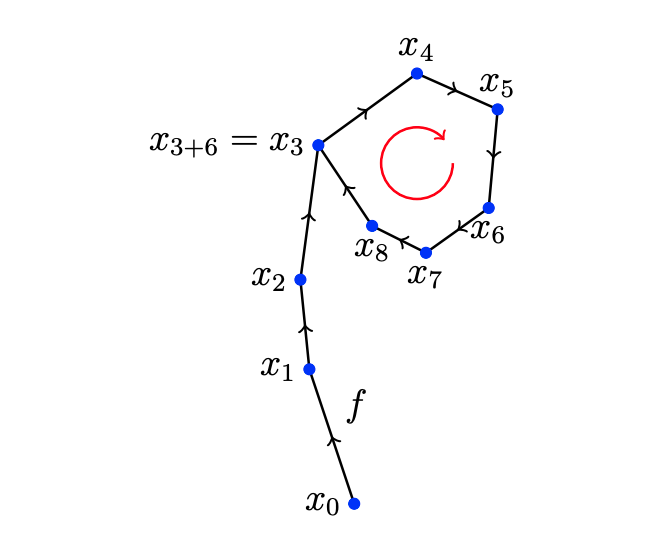
\includegraphics[width=1\textwidth]{rho.png}
 	\caption[Graphical illustration of the Pollard's $\rho$ collision idea]{Graphical illustration of the idea behind the Pollard's $\rho$-algorithm. $T = 3$, the length of the cycle is $M = 6$. Image source: (\cite{mky}, page $70$).}
 	\label{rho}
 \end{figure}
 \end{theorem}
 \begin{theorem}
 The Pollard's $\rho$-algorithm might be used to solve the ECDLP. Let $E(p)$ be an elliptic curve group over a finite field $GF(p)$. Let $P \in E(p)$ and let $Q \in \langle P \rangle$ be another point. We want to find the integer $t=\log_P(Q)$. Let us denote the order of $P$ by $N = \#P$. We divide $\langle P \rangle$ into three disjoint sets $S_1, S_2, S_3$ of approximately the same size. Additionally, we require that $\mathcal{O} \not\in S_2$. For $i \in \mathbb{Z}_{\geq 0}$ we define a function $f: \langle P \rangle \to \langle P \rangle$ as follows:
 $$
 T_{i+1} = f(T_i) := \begin{cases} P \oplus T_i,\quad T_i \in S_1, \\
 2T_i, \quad T_i \in S_2, \\
 Q \oplus T_i, \quad T_i \in S_3.
 \end{cases}
 $$
 We can start with any point in $E(p)$ as long as we know how to express it as a linear combination of points $P,Q$. The usual choice is $T_0 = \mathcal{O} = 0P + 0Q$. After $k$ steps we get:
 $$
 T_k = (\underbrace{f\circ f \circ \cdots \circ f}_\text{$k$-times})(T_0) = \alpha_k P \oplus \beta_k Q.
 $$
 We need to keep track of coefficients $\alpha_k,\ \beta_k$. We start with integers $\alpha_0, \beta_0$, such that $\alpha_0P + \beta_0Q = T_0$ and define the update process recursively:
\begin{align*}
 \forall k \in \mathbb{Z}_{\geq 0}:  \alpha_{k+1} := \begin{cases} \alpha_k + 1\text{ (mod $N$)},\quad &T_k \in S_1, \\
 2\alpha_k\text{ (mod $N$)}, \quad &T_k \in S_2, \\
 \alpha_k, \quad &T_k \in S_3.
 \end{cases} \\
   \forall k \in \mathbb{Z}_{\geq 0}: \beta_{k+1} := \begin{cases} \beta_k,\quad &T_k \in S_1, \\
 2\beta_k\text{ (mod $N$)}, \quad &T_k \in S_2, \\
 \beta_k + 1\text{ (mod $N$)}, \quad &T_k \in S_3.
 \end{cases}
 \end{align*}
We also create a second sequence of points on the elliptic curve $E$: 
$$\forall k \in \mathbb{Z}_{\geq 0}: R_k := T_{2k} = \gamma_kP \oplus \delta_kQ.$$
After a certain number of steps, which we denote by $i$, we encounter a collision: $R_i = T_i$. We then have the following relation: 
$$
\gamma_iP \oplus \delta_iQ = \alpha_iP \oplus \beta_iQ.
$$
Let $d = \text{gcd}(\beta_i - \delta_i, N)$, if $d=1$, then we can easily find the solution $t$ to the ECDLP:
$$
t \equiv (\gamma_i - \alpha_i)\cdot(\beta_i - \delta_i)^{-1} \text{ (mod $N$)}.
$$
If $d \neq 1$, but is small, it might be favourable to find a particular solution $y$ mod($N/d$) in the same fashion:
$$
y \equiv (\gamma_i - \alpha_i)\cdot(\beta_i - \delta_i)^{-1} \text{ $\bigg($mod $\frac{N}{d}\bigg)$}.
$$
Afterwards, we can recover the complete solution $t$ from the set:
$$
\bigg\{y + k\cdot\frac{N}{d}\ \bigg| \ k \in \{0, 1, \ldots, d -1\}\bigg\}.
$$
For $N$ prime $d$ will be small. If $d$ is not small, then we can restart the algorithm with a different partitioning $S_1,S_2,S_3$ or a different starting point $T_0$. Another option is to use the Pohlig-Hellman algorithm and solve multiple ECDLPs in prime order subgroups. Afterwards, we can find the complete solution $t$ using the Chinese remainder theorem (CRT). This idea is refined in subsection \ref{pohlig}.
\end{theorem}
\noindent For example, let $E = E_{11,18}(29)$ be an elliptic curve group over $GF(29)$, defined by the elliptic curve equation is $y^2 = x^3 + 11x + 18$. Let $P = (1,1) \in E$ and let $Q \in \langle P \rangle$ be a second point. We want to find an integer $t$ such that: $Q = tP.$
The order of $P$ is 29 (prime). We divide points of $\langle P \rangle$ into sets $S_1,S_2,S_3$ based on their $x$-coordinates and assign $\mathcal{O}$ to $S_1$:
\begin{align*}
\forall R  \in \langle P \rangle \setminus \{\mathcal{O}\} = (R_x, R_y): \begin{cases} R \in S_1, \quad \text{ if } 0 &\leq R_x < \big\lfloor\frac{p}{3}\big\rfloor, \\ 
R \in S_2, \quad \text{ if } \big\lfloor\frac{p}{3}\big\rfloor &\leq R_x < 2\big\lfloor\frac{p}{3}\big\rfloor, \\
R \in S_3, \quad \text{ if } 2\big\lfloor\frac{p}{3}\big\rfloor &\leq R_x, 
\end{cases}
\end{align*}
where $p = 29.$ Cardinalities of the sets are $|S_1| = 9,\ |S_2| = 12, \ |S_3| = 8.$ 
\\ \\
\noindent \textit{Remark:} There are many different ways how to divide the points into the sets $S_1,S_2,S_3$. The important thing is that the three sets should be approximately of the same size and that for every point $R$ we can efficiently decide to which of the three sets it belongs. \\ \\
\noindent Let us solve the ECDLP with $Q=(13,26)$. In table~\ref{tblRho} are shown the intermediate results of the Pollard's $\rho$-algorithm.
\begin{table}[!h]
\centering
\begin{tabular}{ |c||c|c|c|c|c|c| } 
\hline
$i$ & $\alpha_i$ & $\beta_i$ & $T_i$ & $\gamma_i$ & $\delta_i$ & $R_i$ \\ 
\hline
\hline
0 & 0 & 0 & $\mathcal{O}$ &  0 & 0 & $\mathcal{O}$ \\ \hline
1 & 1 & 0 & $(1,1)$ &  2 & 0 & $(18,25)$ \\ \hline
2 & 2 & 0 & $(18,25)$ &  3 & 1 & $(3,22$ \\ \hline
3 & 2 & 1 & $(5,13)$ &  8 & 2 & $(11,7)$ \\ \hline
4 & 3 & 1 & $(3,22)$ &  3 & 8 & $(8,3)$ \\ \hline
5 & 4 & 1 & $(12,14)$ &  4 & 9 & $(13,3)$ \\ \hline
6 & 8 & 2 & $(11,7)$ &  8 & 19 & $(13,3)$ \\ \hline
7 & 16 & 4 & $(14,4)$ &  16 & 10 & $(13,3)$ \\ \hline
8 & 3 & 8 & $(8,3)$ &  3 & 21 & $(13,3)$ \\ \hline
9 & 4 & 8 & $(26,25)$ &  6 & 14 & $(13,3)$ \\ \hline
10 & 4 & 9 & $\mathbf{(13,3)}$ &  12 & 0 & $\mathbf{(13,3)}$ \\ \hline
\end{tabular}
\caption[Intermediate values of the Pollard's $\rho$-algorithm]{Intermediate values of the Pollard's $\rho$-algorithm.}
\label{tblRho}
\end{table}
\\
\noindent A collision was found after 10 iterations: 
$$
4P + 9Q = 12P \implies t \equiv 8\cdot9^{-1} \text{ (mod $29$)} \equiv 17 \text{ (mod $29$)}. 
$$
We can easily verify that $17P = (13,26) = Q.$
\subsection{Pohlig-Hellman Algorithm}\label{pohlig}
As we have mentioned in the previous subsection, Pollard's $\rho$-algorithm works best in a prime order group. In the case, when the order of the group $G$ is a composite number $N$ with small factors, we can solve multiple ECDLPs in subgroups of prime order. Afterwards, we can use the CRT to find the complete solution. In 1978, Stephen Pohlig and Martin Hellman presented this algorithm in their article~\cite{PH}. 
\begin{theorem}(\textbf{Chinese Remainder Theorem (CRT))}: Let $m_i \in \mathbb{N},\ i \in \{1,\ldots, k\},$ be mutually prime integers, and $N=\prod_{i=1}^k m_i,\ x_i \in \mathbb{Z},\ i \in \{1,\ldots, k\}.$ 
The following system of linear congruences:
\begin{align*}
x &\equiv x_1 \text{ (mod $m_1$)}, \\
x &\equiv x_2 \text{ (mod $m_2$)}, \\
&\vdots \quad \vdots \\
x &\equiv x_k \text{ (mod $m_k$)},
\end{align*}
has a solution $c$:
$$
c = \sum_{i=1}^k x_iN_iM_i \text{ (mod $N$)},
$$ where $N_i=N/m_i$ and $M_i\equiv(N_i)^{-1} \text{ (mod $m_i$)}$. Moreover, any other solution $c'$ is congruent to $c$ modulo $N$.
\end{theorem} 
\begin{theorem}(\textbf{Pohlig-Hellman algorithm}): Let $E(p)$ be an elliptic curve and let $P \in E(p)$ be a point of composite order $N$. Assume $N$ has $k$ distinct prime factors, then the factorisation of $N$ is:
$$
N = \prod_{i=1}^kp_i^{e_i},\ \forall i,j \in \{1, 2, \ldots, k\}: e_i \in \mathbb{Z}_{\geq 0},
$$ where $p_i$ are distinct primes. Let $Q \in \langle P \rangle$, we want to find an integer $x$ such that $xP = Q$. We can split this ECDLP into multiple ECDLPs in the prime power subgroups as follows:
 \begin{itemize}
 \item For each $i \in \{1, 2, \ldots, k\}$ let:
 $$
 P_i := \frac{N}{p_i^{e_i}}P, \quad Q_i := \frac{N}{p_i^{e_i}}Q.
 $$ Each $P_i$ is a generator of a prime power subgroup of $E(p)$. The order of $P_i$ is $\#P_i = p_i^{e_i}.$ We solve an ECDLP in every subgroup $\langle P_i \rangle$, i.e. find an integer $x_i$  such that: $x_iP_i = Q_i.$
 \item  In every prime power subgroup $\langle P_i \rangle$, we may split the ECDLP to $e_i$ ECDLPs in prime subgroups of order $p_i$.  We may rewrite the unknown integer $x_i := y_{i,0} + y_{i,1}p_i + y_{i,2}p_i^2+ \cdots + y_{i,e-1}p_i^{e_i-1}.$ We can now repeatedly solve an ECDLP in a prime subgroup to obtain one unknown digit of $x_i$ at a time, by shifting the rest of them out. To find the first digit $y_{i,0}$ we multiply both sides of the equation by $p_i^{e_i-1}$:
\begin{align*}
p_i^{e_i-1} Q_i &= p_i^{e_i-1}\cdot x_i  P_i\\ 
&= p_i^{e_i-1}\cdot (y_{i,0} + y_{i,1}p_i + y_{i,2}p_i^2+ \cdots + y_{i,e-1}p_i^{e_i-1})P_i \\
&= p_i^{e_i-1}y_{i,0}P_i \oplus p_i^{e_i}\cdot\underbrace{(y_{i,1} + y_{i,2}p_i+ \cdots + y_{i,e-1}p_i^{e_i-2})P_i}_{\in \langle P_i \rangle} \\
&= y_{i,0}p_i^{e_i-1}P_i, \quad \text{(because }\forall T \in \langle P_i \rangle : p_i^{e_i}T = \mathcal{O})
\end{align*}
We may now solve the ECDLP in a prime subgroup of order $p_i$ generated by $p_i^{e_i-1}P_i$, and obtain the first digit $y_{i,0}.$ Afterwards, we move to the next digit $y_{i,1}$ and find it in a similar fashion.
\begin{align*}
p_i^{e_i-2} Q_i &= p_i^{e_i-2}\cdot x_i  P_i\\ 
&= p_i^{e_i-2}\cdot (y_{i,0} + y_{i,1}p_i + y_{i,2}p_i^2+ \cdots + y_{i,e-1}p_i^{e_i-1})P_i \\
&= (p_i^{e_i-2}y_{i,0} + p_i^{e_i-1}y_{i,1})P_i \oplus p_i^{e_i}\cdot\underbrace{y_{i,2}+ \cdots + y_{i,e-1}p_i^{e_i-3})P_i}_{\in \langle P_i \rangle} \\
&= y_{i,0}p_i^{e_i-2}P_i \oplus y_{i,1}p_i^{e_i-1}P_i \implies \\
p_i^{e_i-2}(Q_i \ominus y_{i,0}P_i) &= y_{i,1}p_i^{e_i-1}P_i.
\end{align*}
To find the digit $y_{i,1}$, we need to solve the ECDLP in a prime subgroup of order $p_i$. We continue in the same fashion until all digits of $x_i$ are recovered.
\item Finally we solve the following system of linear congruences:
\begin{align*}
x &\equiv x_1 \text{ (mod $p_1^{e_1}$)}, \\
x &\equiv x_2 \text{ (mod $p_2^{e_2}$)}, \\
&\vdots \quad \vdots \\
x &\equiv x_k \text{ (mod $p_k^{e_k}$)},
\end{align*}
using the CRT to obtain the complete solution $x$.
\end{itemize}
\end{theorem}
\noindent In the individual phase, when solving the ECDLP in a prime order subgroup we can use any algorithm. Usually, BSGS algorithm or Pollard's $\rho$-algorithm is used. The time complexity of Pohlig-Hellman algorithm is therefore (for more information see~\cite{mky}):
$$
O\bigg(\sum_{i=1}^k\bigg[e_i\big(S(p_i) + \log(p_i)\big)\bigg]\bigg),
$$ where $S(p_i)$ is the time complexity of the algorithm used to solve the ECDLP in the prime subgroup of order $p_i$. For elliptic curve groups of composite order with small factors, it is usually more efficient to first run Pohlig-Hellman to split the ECDLP into prime order subgroups, then solve these smaller problems with BSGS or Pollard's $\rho$-algorithm, than to run BSGS or Pollard's $\rho$-algorithm on the original problem. \\\\
\noindent For example, let $E = E_{1,2}(75941)$ be an elliptic curve over the finite field $GF(75941)$, defined by the elliptic curve equation $y^2 = x^3 + x + 2$. Let $P = (64579,62139) \in E$ and let $Q \in \langle P \rangle$ be another point on the elliptic curve $E$. We want to find an integer $x$ such that $Q = xP.$ The order of $P$ is $76428 = 2^2\cdot 3^2\cdot 11 \cdot 193$. Let us solve the ECDLP for $Q = (1447, 50835)$. \\ \\
\noindent We show how the Pohlig-Hellman algorithm solves this ECDLP. 
\begin{table}[H]
\centering
\begin{tabular}{ |c||c|c|c|c|c| } 
\hline
 $i$ & $p_i$ & $e_i$ & $P_i$ & $Q_i$ & $x_i$  \\
\hline
\hline
1 & 2 & 2 & $19107P = (1, 75939)$ &  $19107Q = (1,2)$ & 3  \\ \hline
2 & 3 & 2 & $8492P = (55693, 45178)$ &  $8492Q = (17273,40444)$ & 2 \\ \hline
3 & 11 & 1 & $6948P = (39499, 25804)$ &  $6948Q = (29264,5197)$ & 9 \\  \hline
4 & 193 & 1 & $396P = (58124, 73147)$ &  $396Q = (34502,8697)$ & 189 \\ \hline
\end{tabular}
\caption[Intermediate values of the Pohlig-Hellman algorithm]{Intermediate values of the Pohlig-Hellman algorithm.}
\label{tblPH}
\end{table}
\noindent For $i=1,2$ we need to solve an ECDLP in a subgroup of prime power order. In the subgroup of order $2^2$, generated by $P_1 = (1, 75939)$. We rewrite the unknown partial solution $x_1$ as $x_1 = y_{1,0} + 2y_{1,1}$ and use the following equation to find the first digit $y_{1,0}$:
\begin{align*}
2Q_1 &= y_{1,0}\cdot2P_1 \\
(75940, 0) &= y_{1,0}(75940, 0) \implies y_{1,0} = 1.
\end{align*}
To recover the second digit $y_{1,1}$, we proceed in the similar fashion.
\begin{align*}
Q_1 \ominus y_{1,0}\cdot P_1 &= y_{1,1}\cdot 2P_1 \\
(1,2) \oplus (1,2) & = y_{1,1}(75940, 0) \\
(75940, 0) &= y_{1,1}(75940, 0) \implies y_{1,1} = 1.
\end{align*}
Therefore, $x_1 = y_{1,0} + y_{1,0}\cdot 2 = 1 + 2 = 3.$ In reality, we could have just tried all four possible values of $x_1$. \\ \\
\noindent We repeat the whole process in the subgroup of order $3^2$ generated by $P_2 = (55693, 45178)$. We rewrite the unknown partial solution $x_2$ as $x_2 = y_{2,0} + 3y_{2,1}$ and use the following equation to find the first digit $y_{2,0}$:
\begin{align*}
3Q_2 &= y_{2,0}\cdot 3P_2 \\
(35655, 11621) &= y_{2,0}(35655, 64320) \implies y_{2,0} = 2.
\end{align*}
To find the second digit $y_{2,1}$, we proceed in the similar fashion.
\begin{align*}
Q_2 \ominus y_{2,0}\cdot P_2 &= y_{2,1}\cdot 3P_2 \\
Q_2 \ominus 2P_2 &= y_{2,1}\cdot (35655, 64320) \\
\mathcal{O} &= y_{2,1}\cdot (35655, 64320) \implies y_{2,1} = 0.
\end{align*}
Therefore, $x_2 = 2 + 0\cdot 3 = 2$. In this case, there are nine possible values of $x_2$, which could all have been tried out in the blink of an eye. \\\\
\noindent Now we assemble the system of linear congruences and solve it to find the complete solution $x$.
\begin{align*}
x &\equiv 3 \text{ (mod $4$)}, \\
x &\equiv 2 \text{ (mod $9$)}, \\
x &\equiv 9 \text{ (mod $11$)}, \\
x &\equiv 189 \text{ (mod $193$)}, \\
\end{align*}
\begin{table}[!h]
\centering
\begin{tabular}{ |c||c|c|c|c| } 
\hline
 $i$ & $x_i$ & $m_i$ & $N_i$ & $M_i$ \\
\hline
\hline
1 & 3 & 4 & 19107 &  3 \\ \hline
2 & 2 & 9 & 8492 & 2\\ \hline \hline
3 & 9 & 11 & 6948 & 8 \\ \hline
4 & 189 &193 & 396 & 58 \\ \hline
\end{tabular}
\caption[CRT phase of the Pohlig-Hellman algorithm]{Intermediate values of the CRT phase of the Pohlig-Hellman algorithm.}
\label{tblPH3}
\end{table}
\noindent Using the CRT, we compute $x$ (the intermediate values are in table~\ref{tblPH3}).
\begin{align*}
x &\equiv 3\cdot 19107 \cdot 3 + 2\cdot 8492 \cdot 2 +  9\cdot 6948 \cdot 8 +  189\cdot 396 \cdot 58 \text{ (mod  76428)}\\
 &\equiv 2891\text{ (mod  76428)}.
\end{align*}
We can easily verify that $2891P = (1447, 50835) = Q.$
\section{Index Calculus for the ECDLP}
The Index Calculus is a known \textbf{subexponential} algorithm for solving the DLP in a multiplicative group of a finite field. 
\begin{DF}
Let $0\leq a \leq 1,\ a \in \mathbb{R}$ and $c \in \mathbb{R}_{>0}$. The \textbf{subexponential function} for the parameters $a$ and $c$ is:
$$
L_N(a,c) := \exp(c\log(N)^a \log(\log(N))^{1-a}).
$$
Let $N$ be a $k$-bit integer, note that taking $a=0$ gives $L_N(0,c) = \log(N)^c = k^c$ (polynomial), while taking $a=1$ gives $L_N(1,c) = N^c = \exp(ck)$ (exponential). Thus, $L_N(a,c)$ interpolates exponential and polynomial growth. An algorithm is called \textbf{subexponential} when its complexity is $O(L_N(a,c))$ for some $a$, $0 < a < 1$. For more information see chapter 15 in~\cite{subExp}.
\end{DF} 
\noindent However, it is common to use the name index calculus algorithm to refer to any algorithm that operates in the same fashion as the original Index Calculus algorithm. In other words, an algorithm that solves the DLP by first collecting relations between the group elements, and then using linear algebra to find the complete solution~\cite{amadori17}.
\begin{DF}
\textbf{Index Calculus for ECDLP}: Let $E(p)$ be an elliptic curve group over a prime order field $GF(p)$ and  let $P \in E(p)$. For simplicity, we assume $\#P$ is prime; if that's not the case, then we can use the Pohlig-Hellman idea to split the ECDLP into multiple ECDLPs in prime order subgroups. Let $Q \in \langle P \rangle$ be another point in the subgroup generated by $P$. We want to find an integer $x$ such that $xP = Q$. The simplest version of the index calculus algorithm consists of two main stages, the relation collection step and the linear algebra step. A general index calculus algorithm for solving the ECDLP is described below. First, we need to collect relations.
\begin{enumerate}
\item Specify a factor base $\mathcal{F} \subset \langle P \rangle$, such that we can effortlessly test the membership of an element to this factor base. 
\item Generate a random linear combination $R$ of points $P,Q$.
$$
R := uP + vQ,\quad \text{$u,v$ are random integers in $\{0,1,\ldots ,\#P - 1\}$}.
$$
\item If possible, express $R$ as a linear combination of the elements of the factor base $\mathcal{F}$:
\begin{align*}
&\forall k \in \{1,2,\ldots,|\mathcal{F}|\}: P_k \in \mathcal{F},\ a_k \in \{0,1,\ldots ,\#P - 1\}: \\
&R = uP + vQ = \sum_{k=1}^{|\mathcal{F}|}a_k P_k, \\
&\mathcal{O} = -uP - vQ + \sum_{k=1}^{|\mathcal{F}|}a_k P_k.
\end{align*}
\item If $R$ cannot be expressed in terms of the factor base $\mathcal{F}$, continue with step 2. Otherwise, store the coefficients of $R$ with respect to $\mathcal{F}$ and integers $u,v$ as a row in the relation matrix $M$. The row is stored in this form:
$$
(a_1, a_2, \ldots, a_{|\mathcal{F}|}, -u, -v).
$$
\item We repeat this procedure (steps 2 to 4) until the end condition is met.
\noindent Some authors (see~\cite{amadori17} on page 2) suggest to set the end condition to the number of decomposed points $R$ to be at least $|\mathcal{F}|$. However, we need to state that this condition does not guarantee that the obtained relations are enough to solve the ECDLP. Another option, which guarantees we can solve the ECDLP in the next step, is to collect relations until the rank of the matrix $M$ is $|\mathcal{F}| + 1$. Which is also the maximum rank matrix $M$ can have (assuming $Q \neq \mathcal{O}$).  In section~\ref{alg1} a weaker end condition is stated.
\item After collecting enough relations, the linear algebra step solves the ECDLP. We reduce matrix $M$ to a row echelon form (definition~\ref{rowEch}). Then, the last non-zero row of the reduced matrix looks like $(0,0,\ldots, 0, 1, -v')$, which transforms into the following relation:
\begin{align*}
\mathcal{O}  &= 1P \oplus (-v'Q) \\
P &= v'Q \implies x \equiv (v')^{-1} \text{ (mod $\#P$)}.
\end{align*}
We can always recover the solution $x$ because the order of $\#P$ is prime and $P,Q \neq \mathcal{O} \implies v' \not\equiv 0 \text{ (mod $\#P$)}$.
\end{enumerate}
\end{DF}
\noindent The main bottleneck of this algorithm lies in the decomposition of a point $R$ into the factor basis $\mathcal{F}$, called the \textbf{point decomposition problem (PDP)}. Therefore, in order for this algorithm to be efficient we need to be able to efficiently solve the PDP (including the case when $R$ cannot be decomposed into the elements of $\mathcal{F}$). Additionally, we require a high success rate of the decomposition of $R$ into the factor base $\mathcal{F}$. Both of these requirements are deeply affected by the choice of the factor base $\mathcal{F}$ and its size~\cite{amadori17}. \\ 

\subsection{Summation Polynomials}\label{sumpoly}
\noindent In 2004, Igor Semaev published an article introducing summation polynomials in order to transform the PDP to a problem of finding a solution of a multivariate polynomial equation based on the group law of a specific elliptic curve. This section is based on the original article by Semaev~\cite{semaev04}.
\begin{DF}
Let $E_{A,B}(p)$ be an elliptic curve given by the short Weierstrass equation over a prime field $\mathbb{F} = GF(p),\ p > 3$. For any natural number $n \geq 2$, let $S_n = S_n(X_1, X_2, \ldots, X_n)$ be a polynomial in $n$ variables. We call this polynomial the $n$-th \textbf{summation polynomial} and define it by the following property. Let $x_1,x_2,\ldots,x_n$ be any elements in $\overline{\mathbb{F}}$, the algebraic closure of the field $\mathbb{F}$, then $S_n(x_1,x_2,\ldots,x_n)=0$ if and only if there exist $y_1,y_2,\ldots,y_n \in \overline{\mathbb{F}}$, such that the points $(x_i,y_i), \forall i \in \{1,2,\ldots,n\}$ are in $E(\overline{\mathbb{F}})$, and sum to the identity element of $E_{A,B}(\overline{\mathbb{F}})$.
$$
\sum_{i=1}^n (x_i,y_i) = \mathcal{O}, \quad  \mathcal{O} \in E_{A,B}(\overline{\mathbb{F}}).
$$
\end{DF}
\noindent For $n=2$, the summation polynomial is defined as follows. 
$$
S_2(X_1, X_2) := X_1 - X_2,
$$ it comes from the fact that 
$$
\forall P, Q \in E_{A,B}(\overline{\mathbb{F}}): P \oplus Q = \mathcal{O} \implies  Q = \ominus P.
$$
Based on the definition of the additive inverse in $E_{A,B}(\overline{\mathbb{F}})$, we know the points $P = (x_1,y_1)$ and $\ominus P = (x_1, -y_1)$ have the same $x$-coordinate. Which is equivalent to $S_2(x_1, x_2) = 0 \implies x_1 = x_2.$ 
\\\\
\noindent To determine $S_3(X_1,X_2,X_3),$ let $(x_1,y_1)$ and $(x_2, y_2)$ be two affine ($\neq  \mathcal{O}$) points on $E_{A,B}(\overline{\mathbb{F}})$ such that $x_1 \neq x_2.$ We denote their sum and difference by:
\begin{align*}
(x_3,y_3) &:= (x_1,y_1) \oplus (x_2,y_2),\\
(x_4,y_4) &:= (x_1,y_1) \ominus (x_2,y_2).\\
\end{align*}
We use the group law $\oplus$ to express $x_3$ and $x_4$ in terms of $x_1,x_2, y_1, y_2$.
\begin{align*}
x_3 &= \lambda_3^2 - (x_1 + x_2), \text{ where } \lambda_3 = \frac{y_2 - y_1}{x_2 - x_1},\\ 
x_4 &= \lambda_4^2 - (x_1 + x_2), \text{ where } \lambda_4 = \frac{y_2 + y_1}{x_2 - x_1}, \text{ since } \ominus (x_2,y_2) = (x_2, -y_2).\\ 
\end{align*}
To find a polynomial, such that $x_3$ and $x_4$ are its roots, recall \textbf{Vieta's formulas}. Let $z_1, z_2$ be two roots of a polynomial $p(z) = az^2 + bz + c$. Then the following formulas must be satisfied:
$$
z_1 + z_2 = -\frac{b}{a},\quad z_1z_2 = \frac{c}{a}.
$$
Therefore, we want to express $x_3 + x_4$ and $x_3 x_4$ in terms of $x_1,x_2,A,B$.
\begin{align*}
x_3 + x_4 &= \lambda_3^2 + \lambda_4^2 - 2(x_1+x_2) \\
&= \frac{(y_2-y_1)^2 + (y_2+y_1)^2 -2(x_1+x_2)(x_2-x_1)^2}{(x_2-x_1)^2} \\
&= \frac{2y_2^2+2y_1^2 -2(x_1+x_2)(x_2-x_1)^2}{(x_2-x_1)^2}.
\end{align*}
Substitute for $y_1^2,y_2^2$ using the elliptic curve equation $Y^2 = X^3 + AX + B.$
 \begin{align*}
x_3 + x_4 &= \frac{2(x_1^3+Ax_1+B+x_2^3+Ax_2+B) -2(x_1^3+x_2^3-x_1^2x_2-x_1x_2^2)}{(x_2-x_1)^2},\\
&= 2\frac{(Ax_1+Ax_2+2B) +x_1^2x_2+x_1x_2^2}{(x_2-x_1)^2}, \\
&= 2\frac{x_1(x_1x_2 + A) + x_2(x_1x_2 + A)+2B}{(x_2-x_1)^2},\\ 
&= 2\frac{(x_1 + x_2)(x_1x_2 + A)+2B}{(x_2-x_1)^2}.
\end{align*}
\vphantom{.}
\begin{align*}
\mathsmaller{x_3x_4} &= \mathsmaller{\frac{\big((y_2-y_1)^2 -(x_1^3+x_2^3-x_1^2x_2-x_1x_2^2)\big)\big((y_2+y_1)^2-(x_1^3+x_2^3-x_1^2x_2-x_1x_2^2)\big)}{(x_2-x_1)^4}}, \\
&= \mathsmaller{\frac{\big(y_1^2 + y_2^2 -2y_1y_2 -x_1^3-x_2^3+x_1^2x_2+x_1x_2^2\big)\big(y_1^2 + y_2^2 +2y_1y_2 -x_1^3-x_2^3+x_1^2x_2+x_1x_2^2\big)}{(x_2-x_1)^4}},\\
&= \mathsmaller{\frac{\big(x_1^2x_2 + x_1x_2^2 + Ax_1 + Ax_2 - 2y_1y_2 + 2B\big)\big(x_1^2x_2 + x_1x_2^2 + Ax_1 + Ax_2 + 2y_1y_2 + 2B\big)}{(x_2-x_1)^4}},\\
&= \mathsmaller{\frac{- 4 y_{1}^{2} y_{2}^{2} + x_{1}^{2} x_{2}^{4} + 2 x_{1}^{3} x_{2} A + 4 x_{1}^{2} x_{2}^{2} A + 2 x_{1} x_{2}^{3} A + x_{1}^{2} A^{2} + 2 x_{1} x_{2} A^{2} + x_{2}^{2} A^{2}}{(x_2-x_1)^4}} \\
&+\mathsmaller{ \frac{4 x_{1}^{2} x_{2} B + 4 x_{1} x_{2}^{2} B + 4 x_{1} A B + 4 x_{2} A B + 4 B^{2} + x_{1}^{4} x_{2}^{2} + 2 x_{1}^{3} x_{2}^{3}}{(x_2-x_1)^4}}.
\end{align*}
\vphantom{.}
Substitute for $y_1^2,y_2^2$ using the elliptic curve equation $Y^2 = X^3 + AX + B.$\\
\vphantom{.}
\begin{align*}
x_3x_4 &= \frac{\bigg((x_1-x_2)^2\bigg)\bigg(x_{1}^{2} x_{2}^{2} - 2 x_{1} x_{2} A + A^{2} - 4 x_{1} B - 4 x_{2} B\bigg)}{(x_2-x_1)^4},\\
&= \frac{(x_1x_2-A)^2 - 4B(x_1+x_2)}{(x_2-x_1)^2}.
\end{align*}
Therefore, the $x_3$ and $x_4$ are roots of the polynomial $f(X)$.
\begin{align*}
f(X) :=& (x_2-x_1)^2X^2-2\bigg((x_1+x_2)(x_1x_2 + A) + 2B\bigg)X \\
+& \bigg((x_1x_2-A)^2 - 4B(x_1+x_2)\bigg).
\end{align*}
In the case $x_1=x_2$, one of the points $(x_3,y_3),\ (x_4,y_4)$ is $2(x_1,y_1)$ and the other one has to be $\mathcal{O}$. Without loss of generality, let us consider $(x_3,y_3) = 2(x_1,y_1)$. We show that $x_3$ is the root of the polynomial $f(X)$.
\begin{align*}
x_1 = x_2:\ f(X) &= -2\bigg(2x_1(x_1^2+A)+2B\bigg)X +\bigg((x_1^2-A)^2-8Bx_1\bigg),
\\ X &= \frac{(x_1^2-A)^2-8Bx_1}{4(x_1^3+Ax_1+B)}, \\ 
	X &= \frac{x_1^4-2Ax_1^2-8Bx_1+A^2}{4(x_1^3+Ax_1+B)}.
\end{align*}
Let us express $x_3$ in terms of $x_1,x_2,A,B$.
\begin{align*}
\lambda &= \frac{3x_1^2+A}{2y_1}, \\
	x_3 &= \lambda^2 -2x_1, \\
	x_3 &= \frac{9 x_{1}^{4} + 6 Ax_{1}^{2} + A^{2} -8x_1y_1^2}{4y_1^2}.
\end{align*}
Substitute for $y_1^2$ using the elliptic curve equation $Y^2 = X^3 + AX + B.$
\begin{align*}
x_3 &= \frac{9 x_{1}^{4} + 6A x_{1}^{2} + A^{2}-8 x_{1}^{4} - 8 x_{1}^{2} A - 8B x_{1}}{4(x_1^3+Ax_1+B)} \\
x_3 &= \frac{x_1^4-2Ax_1^2 - 8Bx_1+ A^2}{4(x_1^3+Ax_1+B)}.\\
\end{align*}
The root of $f(X)$ is indeed $x_3$.
Therefore, we define the third summation polynomial as follows:
\begin{align*}
S_3(X_1,X_2,X_3) &:= (X_2-X_1)^2X_3^2-2\bigg((X_1+X_2)(X_1X_2 + A) + 2B\bigg)X_3\\
&+ (X_1X_2-A)^2 - 4B(X_1+X_2).
\end{align*}
$S_3$ is a symmetric polynomial of degree $2$ in each variable $X_1,X_2,X_3$. For more information about summation polynomials see~\cite{semaev04}. In the same article, Semaev also defined a general $n$-th summation polynomial as follows:
\begin{align*}
&\forall k,n \in \mathbb{N},\ n \geq 4,\ n-3\geq k \geq 1:\\
&S_n(X_1,X_2,\ldots, X_n) := \text{Res}_y\bigg(S_{n-k}(X_1,\ldots,X_{n-k-1},y),\ S_{k+2}(X_{n-k},\ldots,X_n,y)\bigg).
\end{align*}
For example, 
\begin{align*}
S_4(X_1,X_2,X_3,X_4) &= \text{Res}_y\bigg(S_3(X_1,X_2,y),\ S_3(X_3,X_4,y)\bigg), \\
S_3(X_1,X_2,y) &= c_0y^2 + c_1y + c_2, \text{ where } \\
c_0 &= (X_2-X_1)^2,\\ 
c_1 &= -2\bigg((X_1+X_2)(X_1X_2 + A) + 2B\bigg),\\
c_2 &=  (X_1X_2-A)^2 - 4B(X_1+X_2),  \\
S_3(X_3,X_4,y) &= d_0y^2 + d_1y + d_2, \text{ where } \\
d_0 &= (X_4-X_3)^2,\\ 
d_1 &= -2\bigg((X_3+X_4)(X_3X_4 + A) + 2B\bigg),\\
d_2 &=  (X_3X_4-A)^2 - 4B(X_3+X_4), \\
S_4(X_1,X_2,X_3,X_4) &= \text{det}
\begin{pmatrix}
c_0 & 0 & d_0 & 0 \\
c_1 & c_0  & d_1 & d_0  \\
c_2 & c_1 &  d_2 & d_1 \\
 0 & c_2 & 0 & d_2 \\
\end{pmatrix}.
\end{align*}
\label{resExample}
\noindent Recall that the resultant of two polynomials with respect to some variable, is zero if and only if both polynomials have a common root (over an algebraically closed field). 
 \\ \\
\noindent We can immediately see the summation polynomials $S_{n-k}(X_1,\ldots,X_{n-k-1},y)$ and $S_{k+2}(X_{n-k},\ldots,X_n,y)$ are tied together by the variable $y$. Because if there exist $x_1,\ldots, x_n, y_0 \in \overline{\mathbb{F}}$ (where $y_0$ is a common root of polynomials $S_{n-k}(y)$ and $S_{k+2}(y)$), satisfying following equations:
$$
S_{n-k}(x_1,\ldots,x_{n-k-1}, y_0) = 0 \land S_{k+2}(x_{n-k},\ldots,x_{n}, y_0) = 0.$$
Then it implies that there exist $P_1,\ldots,P_n, (y_0, y_1) \in E(\overline{\mathbb{F}})$ such that:
\begin{align*}
P_1 \oplus \cdots \oplus P_{n-k-1} \oplus (y_0,y_1) &= \mathcal{O}, \\
\exists v \in \{0,1\}: P_{n-k} \oplus \cdots \oplus P_{n} \oplus (-1)^{v}(y_0,y_1) &= \mathcal{O}, \\
P_1 \oplus \cdots \oplus P_{n-k-1} \oplus (-1)^{v+1}\bigg(P_{n-k} \oplus \cdots \oplus P_{n}\bigg) &= \mathcal{O}.
\end{align*}
Therefore, 
$$
S_n(x_1,\ldots,x_n) = 0.
$$
\\
\noindent Summation polynomials for $n \geq 3,\ n \in \mathbb{N}$, are symmetric, absolutely irreducible and of degree $2^{n-2}$ in each variable $X_i,\ i \in \{1,\ldots,n\}$.
However, the higher degree summation polynomials are hardly practical (compared with $S_3$) because the growth of their degrees (in each variable) is exponential with respect to $n$. In 2015, Semaev himself presented a \enquote{splitting trick}, a way how to transform the $n$-th summation polynomial into a  system of $S_3$ summation polynomials. The splitting trick is based on the resultant properties and the idea of tying multiple polynomial equations together by \textbf{bounding variables}. The constructed polynomial system can be solved more efficiently than a single summation polynomial $S_n$, $n > 3$, for more information see~\cite{semaev15}. 
\begin{theorem}\textbf{(The splitting trick)}: The roots of the $n$-th summation polynomial $S_n(X_1,\ldots,X_n),\ n \in \mathbb{N},\ n > 3,$ in $\overline{\mathbb{F}}[X_1,\ldots,X_n]$ are equivalent to the solutions (in variables $X_1,\ldots,X_n$) to the following polynomial system:
\begin{align*}
&S_3(X_1,X_2,U_1) = 0, \\
&S_3(X_{k+2}, U_{k}, U_{k+1}) = 0, \quad 1 \leq k \leq n-4,\ k \in \mathbb{N}, \\
&S_3(X_{n-1}, X_n, U_{n-3}) = 0.
\end{align*} 
We call variables $U_i,\ i \in \{1, \ldots, n - 3\}$, \textbf{bounding variables}. Therefore, by introducing $n-3$ new variables, we obtain a polynomial system that consists of $n-2$ symmetric polynomials (each only in three variables) of degree two in each of its variables. Instead of a single polynomial in $n$ variables of degree $2^{n-2}$ in each of its $n$ variables.
\end{theorem}
\noindent Summation polynomials reduce the PDP to the solution of a system of multivariate polynomial equations, which are usually solved by calculating the reduced Gröbner basis of the ideal $I$ generated by those polynomials. The set of common zeroes of the polynomials $\in I$ over $\overline{\mathbb{F}}$ is finite. Therefore, the Gröbner basis of~$I$ with respect to the lexicographic monomial order is in triangular form, see definition~\ref{triagForm}. The reduced Gröbner basis of the ideal $I$ is directly calculated with respect to the lexicographic monomial order. Alternatively, it is calculated with respect to another monomial order and then converted using the FGLM algorithm to a Gröbner basis of the same ideal with respect to the lexicographic monomial order, for detailed information about the FGLM algorithm see~\cite{FGLM}. \\ \\
\noindent In the next chapter, we describe three specialised algorithms for solving the ECDLP. 
\chapter{Specialised Algorithms Solving the ECDLP}
\label{specAlg}
In this chapter, we describe three specialised algorithms for solving ECDLP that are based on the theoretical concepts presented in the previous chapters. A detailed complexity analysis of each of the presented algorithms is also given.
\section{Algorithm 1 (Based on Semaev, 2015)} \label{alg1}
Algorithm 1 is based on the Semaev's algorithm proposed in~\cite{semaev15}, few changes had to be made to make the algorithm work for the ECDLP over prime fields $GF(p)$. Semaev's original algorithm works best over prime field extensions where the base field is of small characteristic.  \\ \\
\noindent Let $P \in E(p)$ be a point of prime order $\#P = r,\ p,r$ primes. Let $Q \in \langle P \rangle$ be another point on $E(p)$. We are asked to find an integer $k$ such that $kP = Q.$ Since $\langle P \rangle$ is a finite group of prime order $r$ we are interested in the solution $k\ \text{(mod }r)$. Algorithm 1, which computes this integer $k$, works in multiple steps as described below.
\begin{enumerate}
\item Define the decomposition constant $m \geq 2,\ m \in \mathbb{N},$ and a factor base $\mathcal{F} \subset GF(p)$ of size $\mathlarger{\Big\lceil \sqrt[m]{r} \Big\rceil}$, where $\lceil \cdot \rceil$ is the ceiling function. The factor base $\mathcal{F}$ might consist of $x$-coordinates of random points of the elliptic curve group generated by $P$ (non-deterministic):
$$
\mathcal{F} := \Big\{x\ \Big|\ x \in GF(p),\ \exists y \in GF(p): (x,y) \in \langle P \rangle  \Big\},
$$
or we can take the $|\mathcal{F}|$ smallest $x$-coordinates of points of the elliptic curve group generated by $P$ (deterministic).
\item Construct a relation matrix $M \in GF(r)^{|\mathcal{F}| + 1 \times |\mathcal{F}| + 2}$. Let us order elements of $\mathcal{F}$ and denote the $i$-th element of the factor base $\mathcal{F}$ by $\mathcal{F}_i,$ ${i \in \{0,\ldots,|\mathcal{F}| - 1\}}$.
\begin{align*}
&\begin{matrix}
\hphantom{........}\mathbf{\mathcal{F}_0} & \hphantom{.........} \mathbf{\mathcal{F}_1} & \hphantom{....}\ldots &\hphantom{...} \mathbf{\mathcal{F}_{\mathcal{F} - 1}} & \hphantom{......}\mathbf{u} & \hphantom{........} \mathbf{v}
\end{matrix}\\
M := &\begin{pmatrix}
m_{1,1} & m_{1,2} & \ldots & m_{1,|\mathcal{F}|} & u_1 & v_1 \\
\vdots & \vdots & \cdots & \vdots & \vdots  & \vdots  \\
\hphantom{.}m_{|\mathcal{F}| + 1,1} & m_{|\mathcal{F}| + 1,2} & \ldots & m_{|\mathcal{F}| + 1,|\mathcal{F}|} & u_{|\mathcal{F}| + 1} & v_{|\mathcal{F}| + 1} \hphantom{.}
\end{pmatrix},
\end{align*}
where all elements of the matrix $M$ are in $GF(r)$. Each row of this matrix represents a relation in the group $\langle P \rangle$:
$$
\forall j \in \{1,\ldots,|\mathcal{F}| + 1\}: u_jP \oplus v_jQ \oplus \sum_{i=1}^{\mathcal{F}} m_{j,i} (\mathcal{F}_{i-1}, y_{i-1}) = \mathcal{O}, 
$$
where $y_k,\ k \in \{0,\ldots,|\mathcal{F}| - 1\}$ is the smaller of the $y$-coordinates of the points on $E$ with $x$-coordinate equal to $\mathcal{F}_k$. If there is a point $(\mathcal{F}_k, y)$ in $\langle P \rangle$, then there is also its additive inverse $(\mathcal{F}_k,-y) = (\mathcal{F}_k, p - y)$ in $\langle P \rangle$. We take the smaller of these two values as $y_k := \text{min}(y, p - y)$.  \\ \\
The matrix $M$ is initialized as a zero matrix and we gradually fill it with relations. The row index $rowID$ tells us where to insert the next found relation. We initialize it with $rowID = 1$.
\item For random integers $u,v \in \{0, \ldots, r-1\}$ compute point ${R = uP \oplus vQ.}$ If $R = \mathcal{O}$ and $v \neq 0$ we can immediately solve the ECDLP:
$$k \equiv  (-u)(v)^{-1} \text{ (mod $r$)}.$$ Otherwise, $R$ has affine coordinates $(R_x, R_y)$. If $R_x = \mathcal{F}_k,$ for some $k \in \{0,\ldots,|\mathcal{F}| - 1\},$ then we have a relation which we can add to the relation matrix $M$.
\begin{align*}
M_{rowID,\ k} &=\begin{cases} 1, \quad &R_y < \frac{p}{2}, \\
r-1, \quad &R_y > \frac{p}{2}.
\end{cases}\\
M_{rowID,\ |\mathcal{F}| + 1} &= u_{rowID} = u \text{ (mod $r$)}, \\
M_{rowID,\ |\mathcal{F}| + 2} &= v_{rowID} = v \text{ (mod $r$)}, \\
rowID &= rowID + 1.
\end{align*}
Otherwise, we try to decompose this point as a sum of factor base $\mathcal{F}$ points by solving the following multivariate polynomial system, i.e. we compute $x_1,\ldots,x_m \in \mathcal{F}$ and $u_1,\ldots,u_{m-2} \in GF(p)$ such that:
\begin{align*}
S_3(x_1,x_2,u_1) &= 0, \\
S_3(x_{k+2},u_k,u_{k+1}) &= 0,\quad 1 \leq k \leq m - 3,\ k \in \mathbb{N}, \\
S_3(x_m,R_x,u_{m-2}) &= 0, \\
\Bigg[\prod_{i=0}^{|\mathcal{F}| -1}\Big(x_j - \mathcal{F}_i\Big)\Bigg] &= 0, \quad  j \in \{1, \ldots, m\},
\end{align*}
the last $m$ products are used to restrict the found solutions $x_1,\ldots,x_m$ to lie in the factor base $\mathcal{F}$. Semaev also suggested adding the \textbf{field equations}:
$$
x_j^p - x_j = 0, \quad j \in \{1, \ldots, m\},
$$
which is not computationally feasible for large $p$ (approximately $p \geq 2^{8}$). Therefore, we do not use them in our implementation. Let us denote the set of the polynomials described above as $T$. We can compute the reduced Gröbner basis $G$ of ideal $I = \langle T \rangle$  with respect to lexicographic order $X_1 >_{lex} \cdots >_{lex} X_n$ and by the definition~\ref{triagForm}; $G$ will be in a triangular form. Hence we can easily find the affine variety $\mathcal{V}(G) = \mathcal{V}(T)$, i.e. the set of the common zeroes of the polynomials $\in T$. For every found solution, in variables $X_1,\ldots,X_m$ (we do not care about the values of $u_1,\ldots,u_{m-2}$), ${(s_1, \ldots, s_m),\ s_1,\ldots,s_m \in \mathcal{F}}$; we first determine the signs $o_i,\ i \in \{1,\ldots,m\}$ such that:
$$
\bigg[\sum_{i=1}^m(-1)^{o_i}(s_i, y_i) \bigg] = \mathcal{O}, 
$$
where $y_i = \text{min}(y_i,\ p - y_i)$ is a $y$-coordinate of a point on $E$ with $x$-coordinate equal to $s_i$. After determining the signs $o_i$, we update the matrix $M$ (we start with a row of zeroes):
\begin{align*}
\forall i \in \{1,\ldots,m\}: M_{rowID,\ i} &= M_{rowID,\ i} + \begin{cases} 1, \quad &o_i = 0, \\
r-1, \quad &o_i = 1. \\
\end{cases}\\
M_{rowID,\ |\mathcal{F}| + 1} &= u_{rowID} = u \text{ (mod $r$)}, \\
M_{rowID,\ |\mathcal{F}| + 2} &= v_{rowID} = v \text{ (mod $r$)}, \\
rowID &= rowID + 1.
\end{align*}
\item We repeat step 3, until the end condition is met. The end condition could obviously just be that the matrix $M$ has a full rank $\mathcal{F} + 1$, but in reality we usually need fewer relations. Thus, it is not efficient to always generate that many relations. To solve the ECDLP we just need to transform one row of the matrix $M$ to this form: $(0, \ldots, 0,u',v')$ using only elementary row operations. \\ \\
\noindent Let us denote the matrix $M$ without last two columns by $M'$. We state the end condition as follows. If rank$(M) > $ rank($M')$, then we proceed to step 5. This implies that if we reduce $M$ to its row echelon form, then there will be a leading entry in the $(\mathcal{F} + 1)$-th column of the reduced matrix $M$. We do not consider the degenerate case when $Q = \mathcal{O}$ in which case a leading entry could be in the very last column as well.
\item We reduce $M$ to its row echelon form, as described above and denote it by $M_R$. We can now solve the ECDLP using the last non-zero row of $M_R$ which has to be in the following form:
$$
(0, \ldots, 0, 1, v') \implies P \oplus v'Q = \mathcal{O} \implies k \equiv (-v')^{-1} \text{ (mod $r$)}.
$$
The multiplicative inverse of $(-v')$ always exists because $r$ is a prime number and $P \neq \mathcal{O} \implies v' \not\equiv 0$ (mod $r$). If we denote the rank of the matrix $M$ by~$d$, then the last non-zero row of the matrix $M_R$ is the $d$-th row. \\ Integer $k$ is the solution to the ECDLP.
\end{enumerate}
\subsection{Complexity Analysis of Algorithm 1}
Let us denote the size of the factor base $\mathcal{F}$ by $s = \mathlarger{\Big\lceil \sqrt[m]{r} \Big\rceil}$. The complexity of creating the factor base $\mathcal{F}$ in algorithm 1 is $O(s\cdot \log^3(p))$ because we need to generate $s$ random elements of $\langle P \rangle$ with pair-wise distinct $x$-coordinates. To do that, we can generate a random integer $t$, $0 < t < r$, calculate point $(=t_x, t_y) = tP$ and add $t_x$ to the factor base, we neglect the probability $t_x$ is already in the factor base $\mathcal{F}$. According to table $\ref{tblComp}$, the complexity of calculating $tP$ is $O(\log(t))$ of multiplications in $GF(p)$, which can be bounded by $O(\log^3(p))$ of elementary operations (bit complexity) because $r \leq p + 2\sqrt{p} + 1 \implies O(\log(t)) \approx O(\log(p)).$ \\
\\
\noindent Bit complexity of calculating a random point $R = (R_x, R_y) = aP\ \oplus\ bQ$ is $O(2\log^3(p)) = O(\log^3(p))$. Probability that a random point $R$ can be expressed as:
$$
R = \sum_{i=1}^m(-1)^{o_i}P_i,\quad o_i \in \{0,1\},\ P_i \in \mathcal{F},
$$
is 
$$
2^{m-1}\Bigg(\binom{s}{m}\Bigg)\frac{1}{r} = \frac{2^{m-1}}{r}\frac{(s + m -1)!}{(s-1)!\cdot m!}=\frac{2^{m-1}}{r} \prod_{i=1}^m\frac{(s-1+i)}{i},
$$
where$ \big(\binom{s}{m}\big)$ denotes the number of $m$-combinations with repetition of a set of size $s$. Assuming $m$ is small compared to $s$, we can bound this probability by:
$$
\frac{2^{m-1}}{r\cdot m!} \prod_{i=1}^m(s - 1+i) \leq \frac{2^{m-1}}{r}\frac{s^m}{m!} \approx \frac{2^{m-1}}{m!}.
$$
On average, we need to try $m! / 2^{m-1}$ random points $R$ before we obtain a single relation. Growth of this number with respect to $m$ is shown in the first column of table~\ref{growth}.
\begin{table}[H]
\centering
\begin{tabular}{ |c||c|c| } 
 \hline
 & $m!/2^{m-1}$ & $m^m/2^{m-1}$ \\ 
 \hline
 \hline
$m=2$ & 1& 2\\  \hline
$m=3$ & 1.5 & 6.75\\  \hline
$m=4$ &  3 & 32\\  \hline
$m=5$& 7.5 & 195.31\\ \hline
$m=6$& 22.5 & 1458 \\ \hline
$m=7$& 78.75 & 12868.86  \\ \hline
$m=8$& 315 & 131072  \\ \hline
\end{tabular}
\caption[Decomposition constant $m$ and the average number of tries]{Relationship of the decomposition constant $m$ to the average number of tries before obtaining a single relation.}
\label{growth}
\end{table}
\noindent To simplify our calculations we assume we need to obtain $s$ relations in order to solve the ECDLP. Therefore, we need to calculate $ (s\cdot m!)/(2^{m-1})$ Gröbner bases. \\
\\
\noindent There are at least two main families of Gröbner bases algorithms; the first family is Buchberger's original algorithm and its improvements, the second family are algorithms that transform the problem of computing a Gröbner basis into several instances of Gaussian elimination. Algorithms in the second family are more recent and usually faster, but their computational complexity was not thoroughly examined. Examples of the algorithms in the second family are $F_4, F_5,$ the XL algorithm, and MutantXL, for more information see~\cite{grobComp}. The complexity of these algorithms is dominated by Gaussian elimination in the Macaulay matrix corresponding to the largest degree encountered during the computation, definition of the Macaulay matrix can be found in~\cite{macal}. The number of rows and columns of this matrix depends on the number of variables, the number of polynomials in the system and their degrees. We can bound the complexity of a Gröbner basis computation by those invariants. Let $d$ be the maximum (total) degree reached during a Gröbner basis computation using some algorithm in the second family. There are 
$$
\binom{n+d}{n} = \frac{(n+d)!}{d!\cdot n!} = \prod_{i=1}^{n}\frac{d+i}{i}
$$
monomials, with the leading coefficient equal to 1, in $n$ variables of degree at most $d$. We know that the Gaussian elimination of a $t\times t$ matrix is $O(t^\omega)$, where $2.376 \leq \omega\leq 3$ is a constant. Therefore, we can bound the complexity of a single Gröbner basis computation by:
$$O\Bigg(\bigg(\prod_{i=1}^{n}\frac{d+i}{i}\bigg)^\omega\Bigg).$$
The maximum degree $d$ can be bounded by \textbf{Macaulay bound}, see the corollary 3.26 in~\cite{grobComp}: 
$$d\leq\sum_{f \in I}\text{deg}(f), \quad \text{where $I$ is the input ideal.}$$
This upper bound is quite loose for our case; unfortunately, we were not able to come up with a better one. For the polynomial system in algorithm 1, the number of variables is $2m-2$ as there are $m$ variables $X_i$ and $m-2$ bounding variables $U_j$. The Macaulay bound for this system is: 
$$
d \leq 4(m-1) + m\cdot s,
$$
because there are $m - 1$ summation polynomials $S_3$, which all have total degree $4$, and $m$ bounding polynomials which all have total degree equal to the size of the factor base $\mathcal{F}$, $s = |\mathcal{F}|$. Thus, the complexity of computing a single Gröbner basis of an ideal in algorithm 1 is bounded by:
\begin{align*}
O\Bigg(\bigg(\prod_{i=1}^{2m-2}\frac{(4m-4+m\cdot s + i)}{i}\bigg)^\omega\Bigg).
\end{align*}
Assuming $m$ is significantly smaller than $s$, which is usually the case, then we can simplify this upper bound to:
$$
O\Bigg(\bigg(s^{2m-2}\bigg)^\omega\Bigg) \approx O\bigg(p^{2(\omega -\omega/m)}\bigg).
$$
We need to $s$-times generate a random element $R$, which is $O(\log^3(p))$. As well as approximately $s$-times compute the Gröbner basis of an ideal arising from the step 3. The final step is Gaussian elimination of the relation matrix of size $(s + 1)  \times (s+2)$, which is $O(s^\omega)$. Thus, the complexity of algorithm 1 can be loosely bounded by:
$$
O\bigg(s\cdot\big(\log^3(p) + p^{2(\omega -\omega / m)}\big) + s^\omega\bigg) \approx O\bigg(p^{2(\omega -\omega/m) + 1/m}\bigg).
$$
 \\
 \noindent We conclude that algorithm 1 is exponential in the number of bits of $p$; however, the complexity of computing Gröbner bases of ideals arising from algorithm 1 needs to be better examined. 
\section{Algorithm 2 (Based on Amadori et al., 2017)}
Algorithm 2 is based on the algorithm by Amadori, Pintore and Sala presented in~\cite{amadori17}. The main difference to algorithm 1 is that it uses a factor base with a known decomposition of each of its elements as a linear combination of $P,Q$. Hence, we only require one relation to solve the ECDLP. Algorithm 2 is presented below. \\

\noindent Let $E(p)$ be an elliptic curve group over $GF(p)$ and let $P \in E(p)$ be a point of prime order $\#P = r$. Let $Q \in \langle P \rangle$ be another point in the subgroup generated by $P$. The ECDLP is to find an integer $k$ such that $kP = Q.$ Since $\langle P \rangle$ is a finite group of prime order $r$, we are interested in the solution $k\ \text{(mod }r)$.  Algorithm 2 that solves the ECDLP, works in multiple steps as described below.
\begin{enumerate}
\item Define the decomposition constant $m \geq 3,\ m \in \mathbb{N}$, and a random factor base $\mathcal{F} \subset GF(p)$ of size $\mathlarger{\Big\lceil \sqrt[m]{r} \Big\rceil}$. Elements of the factor base $\mathcal{F}$ are $x$-coordinates of points that are a linear combination of points $P,Q$. Coefficients of each linear combination are stored in the set \textit{coeffs}. Elements of the factor base $\mathbb{F}$ are generated as follows:
\begin{itemize}
\item Start with an empty factor base:
$$
\mathcal{F} := \{\emptyset \}, \quad \textit{coeffs} := \{\emptyset \}.
$$
\item Generate a random point on $E(GF(p))$ as a linear combination of points $P,Q$.
$$
R_i = (x_i, y_i) = a_iP \oplus b_iQ, \quad a_i,b_i \in GF(r),\ r = \#P.
$$
\item If $x_i \not\in \mathcal{F}$, add it to the factor base $\mathcal{F}$ and store the coefficients $a_i,b_i$ of the linear combination in the set \textit{coeffs}.
$$
\mathcal{F} = \mathcal{F} \cup \{x_i\},\quad \textit{coeffs} = \textit{coeffs} \cup \{(a_i, b_i)\}.
$$
\item Repeat the two previous steps until the desired size of the factor base $\mathcal{F}$ is reached.
\end{itemize}
\item Try to find a relation among the factor base points. To find a relation, solve one of the following multivariate polynomial systems: \\
For $t \in \{t_0, \ldots, m\},\ t_0 \geq 3,$ the variables $u_1,\ldots, u_{t - 3}$ are bounding variables.
\begin{align*}
S_3(x_1,x_2,u_1) &= 0, \\
S_3(x_{k+2},u_k,u_{k+1}) &= 0,\quad 1 \leq k \leq t - 4,\ k \in \mathbb{N}, \\
S_3(x_{t-1},x_{t},u_{t-3}) &= 0, \\
f_j(X_j) = \prod_{v \in V_j}(X_j - b) &= 0, \quad j \in \{1, \ldots, t\},
\end{align*}
where $V_j$ are pair-wise disjoint sets of approximately the same size of factor base elements, i.e. $\forall j \in \{1, \ldots, t\}: |V_j| \approx |\mathcal{F}|/t,\ V_j \subset \mathcal{F}.$ The polynomials $f_k$ are used to restrict the solutions $x_1,\ldots,x_t$ to the factor base $\mathcal{F}$. Precisely, each $x_j$ has to lie in the set $V_j$. By splitting the factor base $\mathcal{F}$ into multiple disjoint subsets, we reduce the degree of univariate polynomials in the polynomial system we need to solve.
\item If any of the systems for $t \in \{t_0, \ldots, m\},\ t_0 \geq 3,$ does not have any solutions, we go back to step 1 and use a different factor basis $\mathcal{F}$. If a solution was found, we use it to solve the ECDLP. Assume for some $t \in \{t_0, \ldots, m\},\ t_0 \geq 3$ has a solution $(x_1,\ldots,x_t, u_1, u_{t-3})$, which describes this relation:
$$
\sum_{i=1}^t (-1)^{s_i}(x_i, y_i) = \mathcal{O}.
$$
\end{enumerate}
We recover the signs $s_i,\ i \in \{1, \ldots, t\}$ such that:
\begin{align*}
 i \in \{1, \ldots, t\}: (-1)^{s_i}(x_i,y_i) = R_i &=  a_iP \oplus b_iQ \implies\\
 \sum_{i=1}^t(a_iP \oplus b_iQ) &= \mathcal{O},
 \end{align*}
 where $a_i, b_i$ are coefficients stored in the set \textit{coeffs}. Therefore, the solution $k$ is:
 $$
 k \equiv \bigg(-\sum_{i=1}^t a_i\bigg)\bigg(\sum_{i=1}^t b_i\bigg)^{-1} \text{ (mod $r$)}.
 $$
Solution $k$ is recoverable from this equation, unless $\sum_{i=1}^t b_i \equiv 0 \text{ (mod $r$)},$ which is extremely rare. If that happens, then we need to try a different $t$ or restart the algorithm (from step 1) with a different factor basis.
\subsection{Complexity Analysis of Algorithm 2}
Complexity of a single random factor base $\mathcal{F}$ generation is $O(s\log^3(p))$, where $s = |\mathcal{F}| = \mathlarger{\Big\lceil \sqrt[m]{r} \Big\rceil}$. The reasoning is the same as in the complexity analysis of algorithm 1. We need to generate $s$ elements of a subgroup $\langle P \rangle$ and the complexity of generating one element is $O(\log^3(p))$. By splitting the factor base into $m$ disjoint sets, we reduce the probability of obtaining a relation. On the other hand, we also reduce the degrees of polynomials in our system which significantly reduces the complexity of computing a Gröbner basis of this polynomial system. Probability of obtaining a relation is in this case:
$$
\frac{1}{r}\cdot2^{m-1} \bigg(\frac{s}{m}\bigg)^m \approx \frac{2^{m-1}}{m^m}.
$$
\noindent Based on the fact that the disjoint sets of factor base elements are all about the same size $s/m$. The average number of Gröbner basis computations, in order to obtain a relation, with respect to $m$ is shown in the last column of table~\ref{growth}. \\ \\
\noindent In algorithm 2, we only need to find a single relation.  For the polynomial system in algorithm 2, the number of variables is $2m-3$ because there are $m$ variables $X_i$ and $m-3$ bounding variables $U_j$. Maximum degree $d$ reached during a Gröbner basis computation can be again bounded by Macaulay bound:
$$
d \leq 4(m-2) + s,
$$
because there are $m - 2$ summation polynomials $S_3$, which all have total degree $4$, and $m$ bounding polynomials which all have total degree approximately $s/m$.  Thus, the complexity of computing a single Gröbner basis of an ideal in algorithm 2 is bounded by:
$$
O\Bigg(\bigg(\prod_{i=1}^{2m-3}\frac{4m - 8 + s + i}{i} \bigg)^\omega\Bigg).
$$
Assuming $m$ is significantly smaller than $s$, which is usually the case, we can simplify this upper bound to:
$$
O\Bigg(\bigg(s^{2m-3}\bigg)^\omega\Bigg) \approx O\Bigg( p^{2\omega - 3\omega/m)}\Bigg),
$$
where $\omega$ is $2.376 \leq \omega \leq 3.$
\noindent Therefore, the complexity of algorithm 2 can be bounded by:
$$
O\Bigg(\frac{m^m}{2^{m-1}}\cdot s \cdot p^{2\omega - 3\omega/m} \cdot \log^3(p)\Bigg) \approx O\Bigg(\frac{m^m}{2^{m-1}}\cdot p^{2\omega +(1- 3\omega)/m}\cdot \log^3(p)\Bigg)
$$
We are inclined to believe, although the presented upper bound on the complexity of computing a single Gröbner basis is very loose, that neither of algorithms 1 and 2 is subexponential in the number of bits of $p$. 
\\ \\
\noindent In the original paper \cite{amadori17}, it was incorrectly stated that only one computation of Gröbner basis is needed. In reality, we need to obtain one relation; based on the last column of table \ref{growth} it is evident that only one computation of Gröbner basis is not a realistic assumption. 
\section{Algorithm 3 (Proposed by McGuire et al., 2017)}
Algorithm 3 was proposed by Gary McGuire and Daniela Mueller in \cite{guire}. This algorithm does not use summation polynomials at all, nor does it use Gröbner bases. It tries to find a single relation as does algorithm 2, but algorithm 3 does that by means of exhaustive search. We briefly describe this algorithm in a few steps. \\

\noindent Let $E(p)$ be an elliptic curve defined over the prime order field $GF(p)$ and let $P \in E(p)$ be a prime order element $\#P = r$, $r$ prime. Let $Q \in \langle P \rangle$ be  another point in the subgroup generated by $P.$ We want to find an integer $k$ such that $kP = Q.$ Since $\langle P \rangle$ is a finite group of prime order $r$ we are interested in the solution $k\ \text{(mod }r)$. Algorithm 3 which finds the solution $k$ works in multiple steps as described below.
\begin{enumerate}
\item Define the decomposition constant $m \geq 3,\ m \in \mathbb{N}$, and a random factor base $\mathcal{F} \subset \langle P \rangle$ of size $\mathlarger{\Big\lceil \sqrt[m]{r} \Big\rceil}$. Elements of the factor base $\mathcal{F}$ are linear combinations of points $P,Q$ and the coefficients of each linear combination are stored in the set \textit{coeffs.} Elements of the factor base $\mathcal{F}$ are generated as follows:
\begin{itemize}
\item Start with an empty factor base:
$$
\mathcal{F} := \{\emptyset \}, \quad \textit{coeffs} := \{\emptyset \}.
$$
\item Generate a random point of $R_i \in \langle P \rangle$ as a linear combination of points $P,Q$:
$$
R_i = a_iP \oplus b_iQ, \quad a_i,b_i \in GF(r),\ r = \#P.
$$
\item If $R_i \not\in \mathcal{F}$, add it to the factor base $\mathcal{F}$ and store the coefficients $a_i,b_i$ of the linear combination in the set \textit{coeffs}:
$$
\mathcal{F} = \mathcal{F} \cup \{R_i\},\quad \textit{coeffs} = \textit{coeffs} \cup \{(a_i, b_i)\}.
$$
\item Repeat the two previous steps until the desired size of the factor base $\mathcal{F}$ is reached.
\end{itemize}
\item Try to find a relation among the factor base points. Choose a multiset of $m-1$ points from the factor base, and check whether the \enquote{signed} sum of those points lies in the factor base $\mathcal{F}$. A \textbf{multiset} is a generalisation of the concept of a set that may contain multiple instances of the same element. We denote it by $\{\{ \ldots \}\}.$
Choose a multiset $\{\{P_1, \ldots, P_{m-1} \}\}$ of size $m-1$, where each point $P_i$ lies in the factor base $\mathcal{F}$. Choose signs $\forall i \in \{1, \ldots, m-1\}: o_i \in \{0,1\},$ and let:
$$
P_c := \sum_{i=1}^{m-1}(-1)^{o_i}P_i.
$$
If $P_c \not\in \mathcal{F}$ for all possible choices of signs $o_i$, repeat with another multiset. Else if $P_c \in \mathcal{F}$, go to step 3. If there is no solution for any of the multisets of size $m-1$ of factor base points, go back to step 1 and generate a new factor base $\mathcal{F}$.
\item If $P_c \in \mathcal{F}$, denote $P_m = P_c,\ o_m = 1$, then we have the following relation:
$$
\sum_{i=1}^{m}\Big((-1)^{o_i}P_i \Big) = \mathcal{O}.
$$
\end{enumerate}
We substitute each $P_i$ with $(a_iP \oplus b_iQ)$, using the coefficients stored in the set \textit{coeffs}:
$$
\sum_{i=1}^m(-1)^{o_i}a_i + \sum_{i=1}^m(-1)^{o_i}b_i \equiv 0 \text{ (mod $r$)}, $$
which implies:
$$
k \equiv \bigg(\sum_{i=1}^m(-1)^{o_i + 1}a_i\bigg)\bigg(\sum_{i=1}^m(-1)^{o_i}b_i\bigg)^{-1} \text{ (mod $r$)}.
$$
Solution $k$ is almost always recoverable from this equation. In the unlikely event that $\sum_{i=1}^m (-1)^{o_i}b_i \equiv 0 \text{ (mod $r$)}$, go back to step 2 and try with a different multiset.
\subsection{Complexity Analysis of Algorithm 3}
The complexity analysis of algorithm 3 is based on the original article \cite{guire}.
Denote the size of the factor base $\mathcal{F}$ by $s = |\mathcal{F}|$. The complexity of generating a random factor base of size $s$ is $O(s\log^3(p))$. There is 
$$
\Bigg(\binom{s}{m-1}\Bigg) = \frac{(s + m - 2)!}{(s-2)!\cdot (m-1)!} = \prod_{i=1}^{m-1} \frac{(s -2 + i)}{i}
$$
ways of choosing $m-1$ points from the set $\mathcal{F}$ of size $s$ allowing repetitions. Therefore, there is
 $$
 K:= 2^{m-1}\prod_{i=1}^{m-1} \frac{(s -2 + i)}{i}
 $$
 different ways of forming the sum $P_c = \pm P_1 \pm \cdots \pm P_{m-1},\ P_i \in \mathcal{F},\ i \in \{1,\ldots,m-1\}.$ The complexity of each sum is $O\big((m-2)\log^2(p)\big)$. Probability $P_c \in \mathcal{F}$ is approximately $s/p$, assuming $p \approx \#P$ and assuming the verification whether $P_c \in \mathcal{F}$ is $O(1)$ using a hash-table. Therefore, the complexity of algorithm 3 is bounded by:
 $$
 O\Bigg(\frac{p}{K\cdot s}\bigg( K\cdot\left((m-2)\log^2(p)+ O(1)\right) + s\log^3(p)\bigg)\Bigg),
 $$
where $p/K\cdot s$ is the expected number of different factor bases $\mathcal{F}$ we need to generate. Assuming $m$ is significantly smaller than $s$, we can approximate $K$ by $K \approx 2^{m-1}s^{m-1}/(m-1)!.$ Based on this assumption we can simplify the upper bound of algorithm 3 to:
$$
O\Bigg( \frac{p}{s}(m-2)\log^2(p) + \frac{p\cdot (m-1)!}{2^{m-1}s^{m-1}}\log^3(p)\Bigg) \approx O\Bigg(p^{(m-1)/m}\log^2(p)\Bigg),
$$
assuming $p\cdot \log^3(p)/K$ is $O(p^{(m-1)/m}\log^2(p))$.
\\
\noindent However, for $m=2$ the complexity of algorithm 3 is approximately:
$$
O\Bigg( \frac{1}{2}\sqrt{p}\log^3(p)\Bigg) = O\Bigg(\sqrt{p}\log^3(p)\Bigg)
$$ of bit operations. \\
\chapter{Realisation and Experimental Results}\label{ch4}
In this chapter, we first comment on the choice of a programming language, then provide useful details of the actual implementation that may speed-up the algorithms described in the previous chapter. In the last section, we present the measurements of the performance of our implementation of the algorithms.
\section{Choice of a Programming Language}
Our task was to efficiently implement the three algorithms described in the previous chapter. When choosing a suitable programming language to do so, we had the following things in our minds. We did not want to reinvent the wheel, i.e. implement elliptic curves and operations on them by ourselves. Therefore, we only considered programming languages that have a suitable library for working efficiently with finite fields, polynomial rings and elliptic curve groups. \\
\\ 
\noindent The biggest bottleneck in algorithms 1 and 2 is indisputably the calculation of Gröbner bases. Efficient implementation of Gröbner basis algorithms is an area of active research all over the world. Thus, we have decided to use already existing efficient implementations of Gröbner basis algorithms. There are a few commercial mathematical software packages fulfilling this requirement available, e.g. \textit{Wolfram Mathematica}, \textit{Maple}, \textit{MATLAB}, \textit{Magma} and many more. We must point out \textit{Magma}~\cite{magma}, which is a computational algebra system developed by the scientific community and distributed by the Computational Algebra Group at the University of Sydney, Australia. A lot of other researchers working on the ECDLP use \textit{Magma} to implement their ideas. According to \cite{gbComp}, \textit{Magma} has one of the most efficient implementations of Gröbner basis algorithm $F_4$. There are also some non-commercial alternatives available, e.g. \textit{CoCoA}, \textit{SINGULAR}, \textit{Xcas/Giac}, \textit{SageMath} and many more. \\ \\
\noindent We have opted for \textit{SageMath}, which is a free, open-source mathematics software system, for more information see \cite{sage}. It builds on top of many existing open-source packages, e.g. \textit{CoCoA}, \textit{SINGULAR}, \textit{Xcas/Giac} and many more. We can access their combined power through a common interface using a \textit{Python}-based language. Therefore, it is pretty easy to start with \textit{SageMath}, provided you already have some \textit{Python} experience. Also, \textit{SageMath} and \textit{Python} are available on a broad set of platforms including \textit{Microsoft Windows}, \textit{Linux} and \textit{macOS}. 
\section{Gröbner Basis Algorithms and their Implementations}
The efficiency of both algorithms 1 and 2 is closely related to the efficiency of the Gröbner basis computation. Therefore in this section, we compare different Gröbner bases algorithms and their implementations that are accessible in \textit{SageMath}. \\\\
\noindent \textit{SageMath} uses other mathematical packages to compute Gröbner bases of polynomial ideals. We have compared two algorithms of Buchberger's type implemented in mathematical package called \textit{SINGULAR}. The first variation of Buchberger's algorithm is described in \cite{algGeom} on pages 90--119 and we denote it by \enquote{std}. The second variation is called \enquote{slimgb}, which was developed by Michael Brickenstein and more information is available in~\cite{brick}. We have also tested two implementations of Fauge\`re's $F_4$ algorithm, more details about this algorithm may be found in \cite{algGeom} on pages 567--576. We have tested Fauge\`re's own implementation called \enquote{FGb}, which is licensed for academic use only, more information about \enquote{FGb} can be found in~\cite{fgb}. Since \enquote{FGb} is a \textit{C}-library, we had to use this wrapper \url{https://github.com/mwageringel/fgb_sage} to call its functions directly from \textit{SageMath}. The complexity of the computation greatly depends on the monomial order, we compare $>_{lex}$, $>_{grlex}$ and $>_{grevlex}$ monomial orders using \textit{Giac's} implementation of $F_4$ algorithm.
\\ \\
\noindent We have tested these implementations on problems of different sizes. All tests were carried out on a laptop. The exact configuration of the test machine is described in section~\ref{expResults}. For a problem of each size, determined by the parameter $p$, we have generated 50 polynomial ideals $I \subset GF(p)[x_1,x_2,x_3]$ arising from algorithms 1 and 2. The results shown in table~\ref{gbComp} are averages of our measurements. We denote the number of bits of $p$ by $k =\log_2(p)$. If the monomial order is not specified, the $>_{grevlex}$ order was used. Fauge\`re's \enquote{FGb} supports only finite fields of characteristic $p < 2^{16}$. This fact is denoted by \enquote{NS} when applicable to table \ref{gbComp}. The time limit (TL) was 300 seconds, unfortunately, \enquote{slimgb} was not able to produce results for $p \approx 2^{19}$ in this time limit. The best time in each row is highlighted in bold. All experimental results in table~\ref{gbComp} are in seconds. 
\\ \\
\noindent We can see that \enquote{giac:grevlex} outperformed the other implementations. Therefore, we will use it in our code and we recommend to use it to everyone, who does not have access to \textit{Magma} or \textit{Maple}, which may have even better implementations available. 
\begin{table}[H]
\centering
\begin{tabular}{ |c||c|c|c|c|c|c|c| } 
 \hline
$k$ & \enquote{FGb} & \enquote{giac:lex} & \enquote{giac:grlex} & \enquote{giac:grevlex} & \enquote{slimgb} & \enquote{std} \\ 
 \hline
 \hline
 8 & 0.139 & 0.168 &  0.206 & 0.145 & \textbf{0.119} & 0.121 \\ \hline
10 & 0.168 & 0.210 & 0.189 & \textbf{0.093} & 0.211 & 0.181\\ \hline 
14 & 0.254 & 0.336 & 0.295 & \textbf{0.202} & 0.395 &  0.636 \\ \hline
15 & 1.587 & 2.157 & 1.708 & \textbf{0.896} & 16.45 & 7.231 \\ \hline
16 & 1.876 & 2.466 & 1.654 & \textbf{0.942} & 20.21&  8.87 \\ \hline
19 &  NS & 73.484 & 36.055 & \textbf{16.881} & TL & 266.124  \\ \hline
\end{tabular}
\caption[Comparison of different Gröbner basis algorithms]{Comparison of different Gröbner basis algorithms and their implementations.}
\label{gbComp}
\end{table}
\section{Implementation Remarks}
In this section, we shortly summarize some remarks about our implementation of the algorithms 1, 2 and 3. The source code of our implementation can be found on the attached \textit{CD} in \path{impl/sage/Solve_ECDLP_Matyas_Hollmann.sage}. It is a \textit{SageMath} file, which contains the functions needed for the algorithms to run. To use our implementation, you can simply import the whole file into your \textit{SageMath} notebook/script by:
\begin{lstlisting}[language=Python]
import(.../impl/sage/Solve_ECDLP_Matyas_Hollmann.sage)
\end{lstlisting}
After importing the file into your \textit{SageMath} notebook, you can directly call the functions: \textit{algorithm1Semaev(Q, P, m)}, \textit{algorithm2Amadori(Q, P, m, t0)} and \textit{algorithm3McGuire(Q,P,m)}.
These functions expect the elliptic curve group $\langle P \rangle$ to be a prime order group and that the point $Q$ lies in the subgroup generated by $P$, i.e. it expects that the discrete logarithm $k = \log_P(Q)$ exists. Result $k$ and some statistics about the run are returned to the caller. For more information see the documentation in the source code and the source code itself.
\\ \\
Based on the tests in the previous section, the most efficient open-source library for computing Gröbner bases is \textit{Giac}. Unfortunately, it is not included in the standard installation of \textit{SageMath}. \textit{Giac} is a \textit{C++} library, which can be used directly from \textit{SageMath} via an interface called \textit{Giacpy}. To install \textit{Giacpy} execute the following command in the terminal:
\begin{lstlisting}[language=Python]
sage -i giacpy_sage
\end{lstlisting}
Alternatively, you can download the source code from the GitLab repository: \url{https://gitlab.math.univ-paris-diderot.fr/han/giacpy} and build it yourself. For more information about \textit{Giac/Xcas} see~\cite{giac}.
\\ \\
\noindent We agree on the optimal size of the factor base for algorithms 1 and 2 to be approximately $\sqrt[m]{\#P}$. We have tried increasing the size of the factor base $\mathcal{F}$ to reduce the number of Gröbner bases that need to be computed to obtain a relation. Unfortunately, this led to significantly worse running times. \\ \\
\noindent In algorithm 1, it may be beneficial to check, after new relations are added, whether the column associated to the coefficient $u$ in the relation matrix, would be a leading entry after transforming this matrix to its row echelon form. In \textit{SageMath} we may use the function \textit{M.pivots()}, which returns a list of columns of leading entries of the matrix $M$ in its row echelon form. Our tests showed this to be a useful thing to do. \textit{Giac}'s Gröbner basis algorithm can use multiple threads, on \textit{macOS} it is by default disabled. You can enable the multi-threaded computation of Gröbner basis with the following code snippet:
\begin{lstlisting}[language=Python]
from sage.libs.giac import groebner_basis as gb_giac
import multiprocessing

#on macOS returns number of threads, not CPU count
nthreads = multiprocessing.cpu_count() 

tmp = Ideal(generators) 
gb = gb_giac(tmp, threads=nthreads)
\end{lstlisting}
\hphantom{.}
To get the point $(x,y)$ on the elliptic curve $E$ from its $x$-coordinate, we can use the following function in \textit{SageMath}:
\begin{lstlisting}[language=Python]
point = E.lift_x(x_coord)
\end{lstlisting}
\hphantom{.}
It is advised to implement the factor base $\mathcal{F}$ as a hash-table (dictionary in \textit{Python}) to have a swift look-up operation. Implementation using a hash-table for the factor base in algorithm 3 was more than four times faster than the same implementation using an array for the factor base.
\section{Experimental Results}
\label{expResults}
In this section, we present the measurements of the performance of our implementation of the algorithms and draw a comparison between the three algorithms described in chapter~\ref{specAlg}. All results were obtained on a laptop with the following specifications:  CPU: Intel Core i5 1.3GHz (dual-core, up to 4 threads) with 3MB of shared L3 cache. Operation memory: 4GB 1600MHz LPDDR3. Operation System: 64bit \textit{macOS Mojave} version 10.14.4. Software: \textit{SageMath} version 8.7 with \textit{Giac} version 1.5.0-3 were used. 
\\ \\
\noindent All three algorithms were tested on problems of different sizes. For a parameter $b$ a finite field $GF(p)$ such that $p \approx 2^b$ was generated. A random elliptic curve $E(p)$ such that $\exists P \in E(p)$, $\#P \approx p$ and another point $Q \in \langle P \rangle$ were also randomly generated. Afterwards, the tested algorithm were executed to solve this ECDLP, i.e. to find an integer $k$ such that $kP = Q$. This procedure was repeated multiple times and the results were averaged, the number of repetitions for each problem is stated in the last column of each table. All measured times are in seconds. \\ \\ 
\noindent At first, we have tried to find the optimal parameters for each algorithm with respect to the problem size. The best setting for a problem of each size is highlighted in bold in table~\ref{alg1}. The average number of computed Gröbner bases is in column \enquote{\# GB comp.}.  
\begin{table}[H]
\centering
\begin{tabular}{ |c||c|c|c|c|c| } 
\hline
$b$ & $m$ & \# GB comp. & time$_\text{Sol}$ & \textbf{time}$_\textbf{total}$ & \# repetitions \\
 \hline
 \hline
10 & 2 & 10.54 & 0.638 & \textbf{0.697} & 100 \\ \hline
10 & 3 & 7.52 & 3.001 & 3.103 & 100 \\ \hline
10 & 4 & 10.4 & 6.459 & 6.804 & 100 \\ \hline \hline
11 & 2 & 16.7 & 0.902 & \textbf{0.991} & 100  \\ \hline
11 & 3 & 9.79 & 5.922 & 6.019 & 100  \\ \hline
11 & 4 & 10.8 & 67.514 & 68.090 & 100 \\ \hline
11 & 5	& 9.2 & 138.8 & 139.78 & 100 \\ \hline \hline
12 & 2 & 22.8 & 1.455 & \textbf{1.671} & 100 \\ \hline
12 & 3 & 11.6 & 18.751 & 19.150 & 100 \\ \hline
12 & 4 & 11 & 82.49 & 83.76 & 100 \\ \hline
12 & 5  & 10.4 & 1335.121 & 1337.957 &  25 \\ \hline \hline
13 & 2 & 29.51 & 2.561 & \textbf{2.782} & 100 \\ \hline
13 & 3 & 13.95 & 65.697 & 66.696 & 100 \\ \hline
13 & 4 & 11.2 & 104.322 & 104.987 & 100	\\ \hline \hline
14 & 2 & 40.2 & 4.731 & \textbf{4.987} & 100 \\ \hline
14 & 3 & 17.6 & 234.497 & 236.497 & 100 \\ \hline
14 & 4 & 16.5 & 997.7 & 998.51 & 20 \\ \hline \hline
15 & 2 & 56.31 & 11.387 & \textbf{11.876} & 100 \\ \hline
15 & 3 & 22.125 & 818.421 & 822.251 & 25 \\ \hline \hline
16 & 2 & 72.3 & 22.804 & \textbf{25.405} & 100 \\ \hline
16 & 3 & 29 & 3185.725 & 3186.616 & 15 \\ \hline \hline
17 & 2 & 94.25 & 45.637 & \textbf{50.731} & 100 \\ \hline \hline
18 & 2 & 142.28 & 126.671 & \textbf{142.341} & 100 \\ \hline \hline
19 & 2 & 175.5 & 287.615 & \textbf{322.459} & 100 \\ 
\hline
\end{tabular}
\caption[Experimental results of algorithm 1]{Experimental results of algorithm 1.}
\label{sem}
\end{table}
\noindent The average time (in seconds) spent solving the polynomial systems is in column \enquote{time$_\text{Sol}$}  and the average time (in seconds) of solving the whole ECDLP is in column \enquote{time$_\text{total}$}. As we can see in table~\ref{sem}, the optimal setting for parameter $m$ in algorithm 1 is $m=2$ for small problems. Although the number of Gröbner bases that need to be computed decreases as $m$ increases, the complexity of a single Gröbner basis computation grows significantly faster. Unfortunately, the degree of univariate polynomials, which bound the results to the factor base, is approximately $2^{b/2}$ which is too big for larger values of $b$. Therefore, we recommend using the decomposition constant $m=2$ for small problems. For larger problems, we recommend increasing $m$ to limit the degree of univariate bounding polynomials.
\begin{table}[H]
\centering
\begin{tabular}{ |c||c|c|c|c|c|c| } 
 \hline
$b$ & $t_0$ & $m$ & \# GB comp. & time$_\text{Sol}$ & \textbf{time}$_\textbf{total}$ & \# repetitions \\
 \hline
 \hline
10 & 3 & 3 & 3.79 & 0.061 & \textbf{0.104} & 100 \\ \hline
10 & 4 & 4 & 14.56 & 0.151 & 0.271 & 100 \\ \hline \hline
11 & 3 & 3 & 4.8 & 0.091 & \textbf{0.114} & 100 \\ \hline 
11 & 4 & 4 & 19.31 & 0.191 & 0.435 & 100 \\ \hline \hline
12 & 3 & 4 & 5.14 & 0.112 & \textbf{0.191} & 100 \\ \hline 
12 & 4 & 4 & 15.18 & 0.145 & 0.309 & 100 \\ \hline \hline
13 & 3 & 3& 5.44 & 0.121 & \textbf{0.245} & 100 \\ \hline 
13 & 4& 4 & 19.86 & 0.209 & 0.477 & 100 \\ \hline \hline
14 & 3 & 3 & 6.12 & 0.198 & \textbf{0.371} & 100 \\ \hline
14 & 4 & 4 & 18.75 & 0.252 & 0.583 & 100 \\ \hline \hline
15 & 3 & 3 & 6.77& 0.478 & \textbf{0.745} & 100 \\ \hline 
15 & 4 & 4& 27.29 & 0.805 & 1.49 & 100 \\ \hline \hline
16 & 3 & 3 & 5.06 & 0.823 & \textbf{1.088} & 100 \\ \hline 
16 & 4 & 4 & 24.06 & 1.081 & 1.821 & 100 \\ \hline \hline
17 & 3 & 3 & 5.43 & 2.112 & \textbf{2.479} & 100 \\ \hline 
17 & 4 & 4 & 23.95 & 1.667 & 2.681 & 100 \\ \hline 
17 & 5 & 5& 122.14 & 2.023 & 3.771 & 100 \\ \hline \hline
18 & 3 & 3 & 6.28 & 5.811 & \textbf{6.377} & 100 \\ \hline 
18 & 4 & 4 & 29.33 & 5.875 & 8.341 & 100 \\ \hline
18 & 5 & 5 & 137.1 & 4.791 & 7.221 & 100 \\ \hline \hline
19 & 3 & 3 & 8.2 & 19.081 & 20.711 & 100 \\ \hline 
19 & 4 & 4& 29.5 & 16.312 & \textbf{19.061} & 100 \\ \hline 
19 & 5 & 5 & 188.1 & 16.451 & 20.298 & 100 \\
 \hline
\end{tabular}
\caption[Experimental results of algorithm 2 on small problems]{Experimental results of algorithm 2 on small problems.}
\label{amad1}
\end{table}
\noindent The results of algorithm 2 on small problems $b \leq 19$ are shown in table~\ref{amad1}. It illustrates that the average number of computed Gröbner bases to obtain a single relation is in agreement with the theoretical estimate presented in the last column of table~\ref{growth}. As this number increases, more random factor bases need to be generated. This trend is evident from the comparison of the fourth and fifth columns for different values of $m$.  For larger $m$ algorithm 2 spends more time generating random factor bases than for smaller $m$. The best setting for each problem size is highlighted in bold in table~\ref{amad1}. We recommend to use $m=t_0=3$ for small problems.
\begin{table}[H]
\centering
\begin{tabular}{ |c||c|c|c|c|c|c| } 
 \hline
$b$ & $t_0$ & $m$ & \# GB comp. & time$_\text{Sol}$ & \textbf{time}$_\textbf{total}$ & \# repetitions \\
 \hline
 \hline
20 & 3 & 3 & 4.5 & 29.26 & \textbf{30.1}& 100 \\ \hline
20 & 3 & 4 & 31.9 & 38.12 & 40.10 & 100 \\ \hline 
20 & 4 & 4 & 33.1 & 45.73 & 48.91 & 100 \\ \hline 
20 & 3 & 5& 124.6 & 36.94 & 40.36 & 100 \\ \hline 
20 & 5 & 5 & 140.1 & 34.87 & 38.33 & 100 \\ \hline \hline
21 & 3 & 3 & 5.2 & 110.76 & 115.11 & 100 \\ \hline
21 & 3 & 4 & 20.6 & 93.23 & \textbf{94.87} & 100 \\ \hline
21 & 4 & 4 & 26.3 & 104.1 & 106.21 & 100 \\ \hline
21 & 3 & 5& 133.1 & 144.43 & 148.94 & 100 \\ \hline 
21 & 5 & 5 & 144.13 & 133.12 & 137.51 & 100 \\ \hline \hline
22 & 3 & 3 & 5.0 & 367.83 & 370.87 & 100 \\ \hline
22 & 3 & 4 & 27.8 & 340.71 & 344.21 & 100 \\ \hline
22 & 4 & 4 & 26.9 & 295.22 & 298.33 & 100 \\ \hline 
22 & 3 & 5& 116.4 & 238.27 & 242.71 & 100 \\ \hline 
22 & 5 & 5 & 171.63 & 322.57 & 329.12 & 100 \\ \hline 
22 & 3 & 6 & 863.2 & 152.01 & \textbf{172.15} & 100 \\ \hline \hline
23 & 3 & 3 & 5.9 & 1614.21 & 1617.01 & 15 \\ \hline
23 & 3 & 4 & 40.1 & 1557.11 & 1563.32 & 15 \\ \hline
23 & 4 & 4 & 24.2 & 1345.21 & 1349.2 & 15 \\ \hline 
23 & 3 & 5& 131.4 & 1181.91 & 1209.19 & 15 \\ \hline 
23 & 5 & 5 & 123.1 & 1430.12 & 1446.34 & 100 \\ \hline 
23 & 3 & 6 & 802.1 & 731.12 & \textbf{756.22} & 25 \\ \hline 
\end{tabular}
\caption[Experimental results of algorithm 2 on bigger problems]{Experimental results of algorithm 2 on bigger problems.}
\label{amad2}
\end{table}
\noindent In table~\ref{amad2}, there are results of algorithm 2 on bigger problems: $b \in \{20, 21,$\\ $22, 23\}.$ Although the results are not unequivocal, it seems beneficiary to increase the decomposition constant $m$ and keep $t_0 = 3$. 
\\ \\
\noindent In table~\ref{mcg3}, there are results of algorithm 3 on bigger problems $b\geq 21$. The average number of points $P_c$ that were tried before the relation was obtained is shown in column \enquote{\# points tried}. The average number of factor base $\mathcal{F}$ re-generations is shown in column \enquote{\# restarts}. The other columns have the same meaning as in tables before. \enquote{TL} in the fifth column means that the experiment for the particular parameter setting took too long and was terminated. 
\begin{table}[H]
\centering
\begin{tabular}{ |c||c|c|c|c|c|c| } 
 \hline
$b$ & $m$ & \# points tried & \# restarts & \textbf{time}$_\textbf{total}$ & \# repetitions \\
 \hline
 \hline
21 & 2 & 881 & 0.67 & 4.89 & 100 \\ \hline
21 & 3 & 21886 & 1.25 & \textbf{4.28} & 100 \\ \hline 
21 & 4 & 294546 & 4.1 & 82.22 & 100 \\ \hline \hline 
22 & 2 & 2852 & 1.0 & 9.68 & 100 \\ \hline 
22 & 3 & 39799 & 1.55 & \textbf{7.81} & 100 \\ \hline 
22 & 4 & 378785 & 3.26 & 108.11 & 100 \\ \hline \hline
23 & 2 & 2816 & 0.82 & \textbf{12.97} & 100 \\ \hline
23 & 3 & 92129 & 1.82 & 17.87 & 100 \\ \hline
23 & 4 & 716794 & 3.93 & 189.21 & 100 \\ \hline \hline
24 & 2 & 5467 & 0.94 & \textbf{23.64 }& 100 \\ \hline 
24 & 3 & 201577 & 2.1 & 27.87 & 100 \\ \hline
24 & 4 & 898762 & 3.1 & 211.89 & 100 \\ \hline \hline
25 & 2 & 10697 & 1.05 & 54.85 & 100 \\ \hline 
25 & 3 & 193970 & 1.58 & \textbf{36.71} & 100 \\ \hline 
25 & 4 & 987762 & 2.5 & 345.71 & 100 \\ \hline \hline 
26 & 2 & 7734 & 0.66 & 69.54 & 100 \\ \hline 
26 & 3 & 369541 & 1.92 & \textbf{68.92} & 100 \\ \hline
26 & 4 & 4876649 & 5.2 & 1166 & 15 \\ \hline \hline
27 & 2 & 18328 & 1.14 & 118.22 & 100 \\ \hline 
27 & 3 & 661987 & 2.0 & \textbf{116.14} & 100 \\ \hline 
27 & 4 & - & - & TL & - \\ \hline  \hline
28 & 2 & 24688 & 1 & 289.71 & 100 \\ \hline 
28 & 3 & 510054 & 1.4 & \textbf{157.45} & 100 \\ \hline 
28 & 4 & - &  & TL & - \\ \hline \hline
29 & 2 & 30784 & 0.7 & 437.81 & 100 \\ \hline 
29 & 3 & 1209313 & 1.6 & \textbf{316.14} & 100 \\ \hline 
29 & 4 & - & - & TL & - \\ \hline \hline
30 & 2 & 39762 & 0.8 & 589.23 & 100 \\ \hline 
30 & 3 & 1440651 & 1.4 & \textbf{389.2} & 100 \\ \hline 
30 & 4 & - & - & TL & - \\ \hline \hline
31 & 2 & 61516 & 1.13 & 1879.21 & 15 \\ \hline 
31 & 3 & 3170592 & 1.45 & \textbf{875.8} & 20 \\ \hline 
31 & 4 &- & - & TL & - \\ \hline \hline
32 & 2 & - & - & TL & - \\ \hline 
32 & 3 & 3981245 & 1.54 & \textbf{1023.44} & 15 \\ \hline 
32 & 4 & - & - & TL & - \\ \hline 
\end{tabular}
\caption[Experimental results of algorithm 3]{Experimental results of algorithm 3.}
\label{mcg3}
\end{table}
\noindent It is evident that for this algorithm the optimal parameter setting is $m=3$ for problems $b\geq 21$. We won't publish experimental results of algorithm 3 on smaller problems, but it is better to use parameter $m=2$. These findings are in agreement with the theoretical complexity analysis of algorithm 3 from chapter~\ref{specAlg}. 
\\ \\
\noindent To compare all three presented algorithms with the generic Pollard's $\rho$-algo\-rithm, let us present graph~\ref{grph1}. The horizontal axis represents the problem size in bits~$b$ ($\#P \approx 2^b$). The vertical axis is in logarithmic scale and shows us the time that each algorithm needed to solve the ECDLP with respect to the problem size~$b$. Pollard's $\rho$-algorithm was added to the comparison to illustrate the real efficiency of the algorithms described in the thesis. Graph~\ref{grph1} confirms that all four algorithms (including Pollard's $\rho$-algorithm) are exponential, which is in agreement with our complexity analysis from chapter~\ref{specAlg}. We can also observe that Pollard's $\rho$-algorithm significantly outperforms the other three algorithms.
 \begin{figure}[h]
 \centering
 \hspace*{-1.3cm}
 	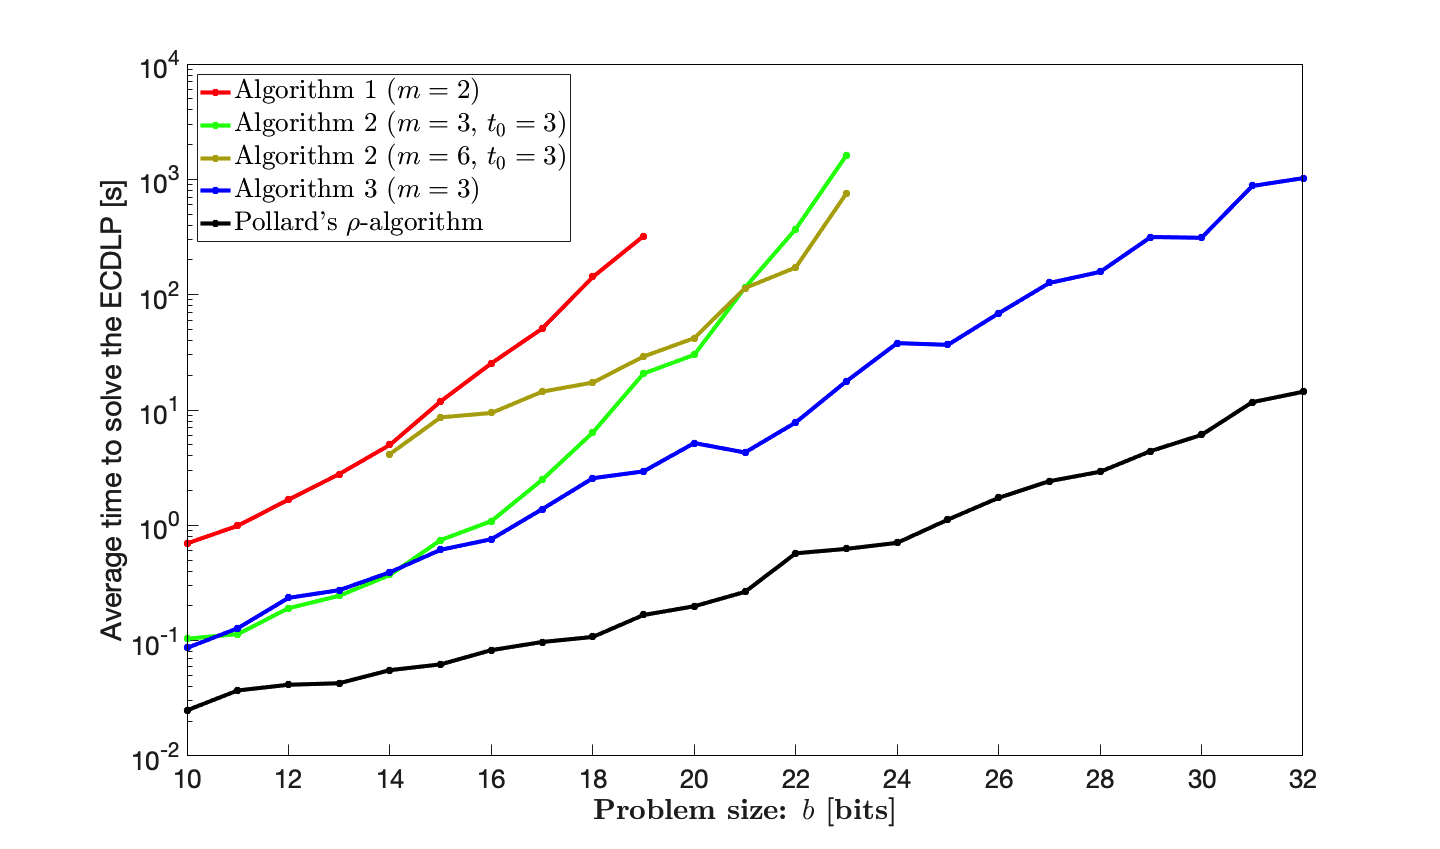
\includegraphics[width=1.21\textwidth]{algComparison.png}
 	\caption[Comparison of different algorithms solving the ECDLP]{Comparison of different algorithms solving the ECDLP.}
 	\label{grph1}
 \end{figure}

\setsecnumdepth{part}
\chapter{Conclusion}
One of the goals of this thesis was to get acquainted with the cryptography of elliptic curves. This goal was fulfilled, and it is described in chapter~\ref{ch2}. The thorough description of summation polynomials and the state-of-the-art algorithms based on them is given in subsection~\ref{sumpoly} and chapter~\ref{specAlg}. The implementation details and experimental results are then available in chapter~\ref{ch4}. \\
\\
\noindent According to our complexity analysis, given in chapter~\ref{specAlg}, of the specialised algorithms solving the ECDLP over a prime field. We need to state that the presented algorithms are unfortunately not yet practical and are easily outperformed by the generic algorithms, e.g. Pollard's $\rho$-algorithm, see graph \ref{grph1}. The theoretical results from chapter \ref{specAlg} are in agreement with our experimental results provided in section~\ref{expResults}. Nevertheless, it is essential to keep trying new approaches for solving the ECDLP. To make these algorithms viable, more research needs to be done in this field. The complexity of Gröbner basis computation of ideals arising in algorithms 1 and 2 also needs to be better understood. The main result of this thesis is the confirmation that the presented algorithms are not competitive with generic algorithms over prime fields. Additionally, an efficient implementation in \textit{SageMath} of said algorithms is available to everyone concerned.
%\bibliographystyle{iso690}
%\bibliography{bibliography}
\begin{thebibliography}{10}

%\bibitem{Abel} THE EDITORS OF ENCYCLOPAEDIA BRITANNICA. \textit{Niels Henrik Abel: NORWEGIAN MATHEMATICIAN.} Encyclopaedia Britannica [online]. Apr 2, 2019 [Accessed on 2019-04-10]. Available at: \url{https://www.britannica.com/biography/Niels-Henrik-Abel}

\bibitem{algGeom} {COX, David A., John LITTLE and Donal O'SHEA. \textit{Ideals, Varieties, and Algorithms: An Introduction to Computational Algebraic Geometry and Commutative Algebra.} Fourth Edition. New York: Springer, 2015. Undergraduate texts in mathematics. ISBN 978-3-319-16721-3.}

\bibitem{mky} {KALVODA, Tomáš, Ivo PETR and Štěpán STAROSTA. Matematika pro kryptologii [online]. KAM FIT ČVUT. [Praha], Updated on 20-02-2019 [Accessed on 16-04-2019]. Available at: \url{https://courses.fit.cvut.cz/MI-MKY/media/lectures/mi-mky-poznamky-v17.pdf}}

\bibitem{myBP} {HOLLMANN, Matyáš. \textit{Implementace násobení na neasociativních (nekomutativních) algebrách.} Praha, 2017. Bakalářská práce. České vysoké učení technické v Praze, Fakulta informačních technologií. Vedoucí práce Jiřina Scholtzová. Available at: \url{https://dspace.cvut.cz/bitstream/handle/10467/69263/F8-BP-2017-Hollmann-Matyas-thesis.pdf}}

\bibitem{coset}{BRAY, Nicolas. \textit{Coset}. From MathWorld-A Wolfram Web Resource [online], created by Eric W. Weisstein. [Accessed on 16-04-2019]. Available at : \url{http://mathworld.wolfram.com/Coset.html}}

\bibitem{handbook}{COHEN, Henri, Gerhard FREY and Roberto AVANZI. \textit{Handbook of elliptic and hyperelliptic curve cryptography.} Boca Raton: Taylor and Francis, 2006. ISBN 978-1-58488-518-4.}


\end{thebibliography}
%citace

\setsecnumdepth{all}
\appendix

\chapter{Acronyms}
% \printglossaries
\begin{description}
	\item[RSA] Rivest-Shamir-Adleman (cryptosystem)
	\item[ECC] Elliptic curve cryptography
	\item[SEA] Schoof-Elkies-Atkin’s (algorithm)
	\item[DLP] Discrete logarithm problem
	\item[ECDLP] Elliptic curve discrete logarithm problem
	\item[EEA] Extended Euclidean algorithm
	\item[BSGS] Baby-step giant-step (algorithm)
	\item[CRT] Chinese remainder theorem
	\item[PDP] Point decomposition problem
	\item[TL] Time limit
\end{description}


\chapter{Contents of Enclosed CD}

\begin{figure}
	\dirtree{%
		.1 readme.txt\DTcomment{the file with CD contents description}.
		.1 impl\DTcomment{the directory of source codes}.
		.2 sage\DTcomment{implementation sources}.
		.2 latex\DTcomment{the directory of \LaTeX{} source codes of the thesis}.
		.1 text\DTcomment{the thesis text directory}.
		.2 DP\_Hollmann\_Matyas\_2019.pdf\DTcomment{the thesis text in PDF format}.
	}
\end{figure}

\end{document}
